\documentclass[11pt]{article}
\usepackage[margin=1in]{geometry}
\usepackage{amsmath,amssymb,booktabs,array,enumitem,graphicx,xcolor,float,hyperref}
\usepackage[nameinlink,noabbrev]{cleveref}
\hypersetup{colorlinks=true,linkcolor=blue,citecolor=blue,urlcolor=blue,hypertexnames=false}
\setlength{\emergencystretch}{2em}

\newcommand{\z}{z}
\newcommand{\psiT}{\psi}
\newcommand{\Htd}{H_{\mathrm{TD}}}

\title{Graph-Assisted Latent MPC: GAS subgoals and cost-to-go inside LeWM's CEM planner\\
\large Working notes and results log}
\author{Mayaank Ashok}
\date{September 2026 (living document; \texttt{results\_table.tex} is regenerated by \texttt{scripts/gas\_mpc\_report.py})}

\begin{document}
\maketitle

\paragraph{Current scope (2026-09-17).} The active project is graph-assisted planning
inside LeWM's CEM planner, with frozen LeWM dynamics and CEM as the low-level controller.
TDR/graph construction, subgoal and cost-to-go objectives, viability or expected-hitting-time
terms, and the final-goal switch are the current research mechanisms. Earlier IQL/GCIQL
actors, graph-derived auxiliary-value regression, reward shaping, and GAS with a learned
low-level policy are historical context, not active development directions. References to
those experiments below explain the motivation for the CEM study and preserve their results.

\section{Question}
LeWM's planner scores a candidate action sequence by the terminal latent L2 distance
$\|\z_T - \z_g\|^2$ between the predicted endpoint and the goal latent, then executes the
CEM optimum receding-horizon (5 blocks of 5 env steps, replanned every 25 steps). It reaches
same-episode goals 25 steps ahead 90--94\% of the time, 50 steps ahead about 60\%, and an
arbitrary goal drawn from a \emph{different} episode only 10.8\% of the time (250 fixed pairs,
5 seeds; seed~0 alone: 4\%). Earlier audits located the failure in the objective: latent L2
stops ranking candidates correctly past $\sim$50 steps (Spearman vs.\ a privileged oracle
0.72 at offset 25, 0.36 at offset 50).

Graph-Assisted Stitching (GAS, Baek et al., ICML 2025) replaces a learned high-level policy
with shortest-path search on a graph built in a Temporal Distance Representation (TDR)
$\psiT$, where $\|\psiT(s)-\psiT(g)\|\approx$ the minimum number of steps from $s$ to $g$.
Its subgoals are, by construction, within $\Htd$ steps of the current state---inside the
range where a local controller's cost is trustworthy. This document asks whether the
same construction, consumed by LeWM's CEM planner instead of a learned low-level policy,
moves the cross-episode and long-horizon numbers. The RL version of GAS on the same latent
(see \texttt{outputs/gas\_pusht}) found the low-level policy, not the graph, was the win;
CEM is a much stronger low-level controller (90\% vs.\ 51\% at offset 25), so this is a
cleaner test of the graph itself.

\paragraph{Answer in one paragraph.} The graph subgoal one horizon ahead repairs the mid-range
regime on its own (offset 50: 40 $\to$ 58\%) but not arbitrary goals; the viability critic as a
feasibility term is what turns the graph's route into cross-episode successes. Composed
naively ($-\log V$, per-population standardisation, goal switch at $\Htd$) the critic lost
8--13 points at offset 25 and needed a different weight $\beta$ per protocol. Two changes fix
both (phase 8, \cref{sec:phase8}): plan the final horizon straight at the goal with LeWM's own
L2 once the goal is within one lookahead, and replace $-\log V$ by a budget-capped expected
hitting time. The resulting single configuration (\textbf{OUR}) is at or above every alternative
on every protocol: \textbf{90.8 / 64.4 / 50.4 / 44.4\%} at same-episode offsets 25 / 50 / 100
and cross-episode over five seeds (250 (task, seed) pairs per protocol), against L2's
91.2 / 48.4 / 11.2 / 10.4 on the same pairs.

\section{Setup}
\paragraph{Data.} All 18,685 Push-T expert episodes (2,336,736 frames), encoded once with
the frozen LeWM encoder (CLS latent, 192-d) by \texttt{scripts/gas\_mpc\_prepare.py encode}.
Approximately 2\% of episodes (373, using integer truncation) are held out from TDR
training and default graph construction. Historical evaluation pools draw from the full
dataset; the new held-out task convention below uses only these excluded episodes.

\paragraph{TDR.} $\psiT:\mathbb{R}^{192}\to\mathbb{R}^{32}$, a 3$\times$512 LayerNorm/GELU
MLP on the frozen latent, trained with the HILP/GAS expectile-TD loss (expectile 0.99,
$\gamma=0.99$, goal relabelling 0.625 same-trajectory / 0.375 uniform, two-member target
min), 50k steps of batch 1024. Diagnostics: Spearman of $\|\psiT(s)-\psiT(g)\|$ vs.\ the
privileged state-distance oracle on held-out cross pairs, Spearman vs.\ the true step gap
on same-episode pairs, and the median TDR distance per step gap (the calibration that says
what one TDR unit is in env steps).

\paragraph{Graph.} Paper Alg.~2 with the official code's conventions: TE filter at
$\theta_{\mathrm{TE}}\ge 0.9$, TD-aware sequential clustering at radius $\Htd/2$ (GPU
implementation, verified bit-identical to the sequential reference), edges between nodes
within $\Htd$ with weight = TDR distance, goal attached as a temporary node linked to every
node within $\max(\Htd, 1.2\cdot d_{\min})$. Each node also carries the latent $\z$ of its
medoid frame so it can serve as a goal for the L2 cost.

\paragraph{Planner.} Unchanged LeWM CEM (300 samples, 30 iterations, top-30, horizon 5
blocks, receding 5 blocks, seeded). Only \texttt{model.criterion} is replaced. The
criterion sees the current latent $\z_0$, the five predicted block latents
$\hat\z_1..\hat\z_5$ (5, 10, \dots, 25 env steps ahead) and the goal latent $\z_g$.

\paragraph{Objectives.} With $h(\cdot)=\psiT(\cdot)$, $D_g[v]$ the Dijkstra distance from
node $v$ to the attached goal, and $c_v$ the node centres:
\begin{itemize}[nosep]
  \item \textbf{l2}: $\|\hat\z_5-\z_g\|^2$ (LeWM).
  \item \textbf{tdr}: $\|h(\hat\z_5)-h(\z_g)\|$ (temporal metric, no graph).
  \item \textbf{ctg}: $\min\big(\|h(\hat\z_5)-h(\z_g)\|,\ \min_v \|h(\hat\z_5)-c_v\|+D_g[v]\big)$
        (graph cost-to-go as a terminal value; no subgoal commitment).
  \item \textbf{subgoal}: Alg.~1 picks $v^\star=\arg\min_{v:\|h(\z_0)-c_v\|\le\Htd} D_g[v]+\|h(\z_0)-c_v\|$,
        then walks the shortest path toward the goal until the cumulative TDR distance from
        $\z_0$ reaches \texttt{lookahead}; cost $=\|\hat\z_5-\z_{\mathrm{med}(v^\star)}\|^2$;
        the true goal once $\|h(\z_0)-h(\z_g)\|\le\Htd$.
  \item \textbf{subgoal\_tdr}: the same node, cost $\|h(\hat\z_5)-c_{v^\star}\|$.
  \item \textbf{dir}: $-\langle h(\hat\z_5)-h(\z_0),\ \vec h_{\mathrm{dir}}\rangle$ with
        $\vec h_{\mathrm{dir}}$ the unit direction to $c_{v^\star}$ (the paper's $r^{\mathrm{dir}}$
        summed over the horizon); \textbf{tdr} once within $\Htd$ of the goal.
  \item \textbf{path}: $\sum_{k=1}^{5}\|h(\hat\z_k)-w_k\|$ with waypoints $w_k$ the path
        nodes at cumulative TDR distance $k\cdot u_5$ from $\z_0$ ($u_5$ = the calibrated
        TDR distance of a 5-step gap), the goal once the path ends.
\end{itemize}

\paragraph{Final-phase switch and critic terms (phase 8).} The subgoal objectives switch
to the true goal once $\|h(\z_0)-h(\z_g)\|\le\theta_{\mathrm{final}}$. The default
$\theta_{\mathrm{final}}=\Htd$ (8 units, $\approx$12 steps) still targets a cluster medoid on
the first solve of a 25-step task; \texttt{final\_thresh}=13.7 (one lookahead $\approx$ 25
steps) plans the whole final horizon at the goal, and \texttt{final\_metric=l2} scores that
phase with LeWM's $\|\hat\z_5-\z_g\|^2$ instead of the TDR norm. The viability critic
$V(\z,\z_g,h)$ (\texttt{outputs/pusht/critic\_training/critic\_full\_sN}, with $N$ the seed) enters through one of:
\begin{itemize}[nosep]
  \item \textbf{nlv}: $-\log V(\hat\z_5,\z_g,h_{\mathrm{rem}})$, $h_{\mathrm{rem}}$ the budget
        left after the plan being scored (\texttt{PlanClock}), clipped to the critic's $h_{\max}=50$.
  \item \textbf{ET}: $5\sum_{h\in\{0,5,\dots,h_{\mathrm{rem}}\}}\big(1-V(\hat\z_5,\z_g,h)\big)$,
        a budget-capped expected hitting time in env steps: feasible endpoints are ordered by
        how soon they arrive, infeasible ones sit at the cap.
\end{itemize}
and is composed with the base cost $c$ as either \textbf{std}: $\tilde c+\beta\,\tilde V$ with
$\tilde x=(x-\mathrm{med}\,x)/\mathrm{IQR}\,x$ over the 300 CEM candidates of each env;
\textbf{steps}: $\mathrm{steps}(c)+\beta\,\mathrm{ET}$ with no standardisation, where
$\mathrm{steps}(\cdot)$ inverts the empirical median-distance-by-step-gap table (TDR units or
z-space L2, gaps 1--50, \texttt{gap\_calib\_s\{seed\}.json}) so both terms are in env steps
and $\beta=1$ is the nominal weight; or \textbf{filter}: rank by $c$ among candidates with
$V(\hat\z_5,\z_g,h_{\mathrm{rem}})\ge\tau$, by $V$ alone when none pass (no weight).

\paragraph{Protocol.} Fixed (start, goal) pairs, identical for every objective:
\texttt{outputs/pusht/critic\_training/cross\_episode/pairs\_*.json}
(generated from \texttt{default\_rng(seed)} alone). Same-episode offset $K$: budget $2K$
(capped at 250). Cross-episode: budget 250. Success = the env's own \texttt{terminated}
(agent+block position error $<20$\,px and block angle error $<\pi/9$). Single seed, 50
pairs per protocol, for screening; promising objectives get more seeds and pairs.

\section{Final Results}
\label{sec:final-results}
Headline comparison, LeWM's own terminal L2 vs.\ the winning configuration
\textbf{OUR} (\texttt{subgoal\_tdr} $+$ final-goal switch at one lookahead $+$ z-space L2 in
the final phase $+$ the budget-capped expected-hitting-time critic term, $\beta=1$;
\cref{sec:phase8}), across all three environments and every goal protocol, on the current
held-out, disjoint \texttt{task200u} pool with planning and critic assets prepared from
training episodes only (\cref{sec:task-pools,sec:task-critic-refresh}). Each cell is the
5-seed mean $\pm$ sd on the fixed 200-task pool (first 50 tasks used), same tasks and same
CEM seeds for L2 and OUR.

\begin{table}[H]
\centering\small
\caption{Push-T, held-out \texttt{task200u} pool, training-only planning/critic assets.
OUR+retr adds demonstration retrieval (\cref{sec:cube-variants}) to OUR's exact
configuration; unlike Cube (below), it does not help here.}
\label{tab:pusht-summary}
\begin{tabular}{lrrrr}
\toprule
configuration & same-ep 25 & same-ep 50 & same-ep 100 & cross-ep \\
\midrule
random & 4.0 $\pm$ 1.3 & 0.4 $\pm$ 0.8 & 0.0 $\pm$ 0.0 & 0.4 $\pm$ 0.8 \\
l2 & \textbf{91.2} $\pm$ 1.0 & 40.8 $\pm$ 3.7 & 13.2 $\pm$ 3.2 & 14.4 $\pm$ 3.9 \\
OUR & 88.4 $\pm$ 2.3 & \textbf{70.0} $\pm$ 2.2 & \textbf{46.4} $\pm$ 3.2 & \textbf{42.4} $\pm$ 3.2 \\
OUR+retr & 86.8 $\pm$ 2.0 & 66.8 $\pm$ 5.2 & 44.8 $\pm$ 4.7 & \textbf{42.4} $\pm$ 6.2 \\
\bottomrule
\end{tabular}
\end{table}

\begin{table}[H]
\centering\small
\caption{Reacher, held-out \texttt{task200u} pool, training-only planning/critic assets.
OUR+retr adds demonstration retrieval (\cref{sec:cube-variants}) to OUR's exact
configuration; as on Push-T, it hurts here.}
\begin{tabular}{lrrrr}
\toprule
configuration & same-ep 25 & same-ep 50 & same-ep 100 & cross-ep \\
\midrule
random & 8.0 $\pm$ 3.8 & 8.4 $\pm$ 0.8 & 9.2 $\pm$ 3.2 & 2.8 $\pm$ 1.0 \\
l2 & \textbf{77.2} $\pm$ 4.8 & 90.8 $\pm$ 1.0 & 82.8 $\pm$ 1.0 & 29.2 $\pm$ 2.4 \\
OUR & 76.0 $\pm$ 4.6 & \textbf{98.0} $\pm$ 1.3 & \textbf{97.6} $\pm$ 0.8 & \textbf{65.6} $\pm$ 2.0 \\
OUR+retr & 62.0 $\pm$ 6.4 & 88.4 $\pm$ 2.7 & 94.0 $\pm$ 1.3 & 63.6 $\pm$ 2.3 \\
\bottomrule
\end{tabular}
\end{table}

\begin{table}[H]
\centering\small
\caption{Cube, held-out \texttt{task200u} pool, training-only planning/critic assets.
OUR+retr adds demonstration retrieval (\cref{sec:cube-variants}) to OUR's exact
configuration; Cube-only, not part of the 3-environment headline comparison.}
\begin{tabular}{lrrrr}
\toprule
configuration & same-ep 25 & same-ep 50 & same-ep 100 & cross-ep \\
\midrule
random & 21.2 $\pm$ 3.0 & 12.8 $\pm$ 2.0 & 4.8 $\pm$ 4.1 & 3.6 $\pm$ 2.3 \\
l2 & 56.0 $\pm$ 3.8 & 34.4 $\pm$ 3.2 & 35.6 $\pm$ 1.5 & 16.4 $\pm$ 1.5 \\
OUR & 62.0 $\pm$ 4.7 & 49.6 $\pm$ 4.6 & 50.4 $\pm$ 3.2 & 27.6 $\pm$ 6.1 \\
OUR+retr & \textbf{86.4} $\pm$ 4.1 & \textbf{59.2} $\pm$ 2.4 & \textbf{78.8} $\pm$ 3.0 & \textbf{48.0} $\pm$ 2.8 \\
\bottomrule
\end{tabular}
\end{table}

\subsection*{Per-seed results}
Every cell above, broken down by seed. ``solved'' = tasks (out of 50) solved in
$\geq$1 of the 5 CEM seeds / solved in every one of the 5 seeds.

\begin{table}[H]
\centering\small
\caption{Push-T, per seed, held-out \texttt{task200u} pool. OUR+retr adds demonstration
retrieval to OUR's exact configuration (\cref{sec:cube-variants}); it does not help on
Push-T, unlike Cube.}
\begin{tabular}{llrrrrrrr}
\toprule
protocol & configuration & s0 & s1 & s2 & s3 & s4 & mean $\pm$ sd & solved \\
\midrule
same-ep 25 & random & 2 & 4 & 4 & 4 & 6 & 4.0 $\pm$ 1.3 & 7 / 0 \\
same-ep 25 & l2 & 92 & 92 & 90 & 92 & 90 & 91.2 $\pm$ 1.0 & 47 / 43 \\
same-ep 25 & OUR & 86 & 88 & 90 & 86 & 92 & 88.4 $\pm$ 2.3 & 48 / 39 \\
same-ep 25 & OUR+retr & 88 & 90 & 84 & 86 & 86 & 86.8 $\pm$ 2.0 & 48 / 34 \\
\midrule
same-ep 50 & random & 0 & 0 & 0 & 2 & 0 & 0.4 $\pm$ 0.8 & 1 / 0 \\
same-ep 50 & l2 & 34 & 40 & 42 & 44 & 44 & 40.8 $\pm$ 3.7 & 28 / 15 \\
same-ep 50 & OUR & 72 & 72 & 70 & 70 & 66 & 70.0 $\pm$ 2.2 & 47 / 21 \\
same-ep 50 & OUR+retr & 74 & 62 & 72 & 64 & 62 & 66.8 $\pm$ 5.2 & 44 / 13 \\
\midrule
same-ep 100 & random & 0 & 0 & 0 & 0 & 0 & 0.0 $\pm$ 0.0 & 0 / 0 \\
same-ep 100 & l2 & 18 & 14 & 14 & 12 & 8 & 13.2 $\pm$ 3.2 & 15 / 2 \\
same-ep 100 & OUR & 48 & 44 & 52 & 44 & 44 & 46.4 $\pm$ 3.2 & 41 / 9 \\
same-ep 100 & OUR+retr & 48 & 48 & 36 & 48 & 44 & 44.8 $\pm$ 4.7 & 42 / 5 \\
\midrule
cross-ep & random & 0 & 0 & 0 & 0 & 2 & 0.4 $\pm$ 0.8 & 1 / 0 \\
cross-ep & l2 & 14 & 14 & 8 & 16 & 20 & 14.4 $\pm$ 3.9 & 16 / 1 \\
cross-ep & OUR & 38 & 42 & 48 & 42 & 42 & 42.4 $\pm$ 3.2 & 35 / 6 \\
cross-ep & OUR+retr & 34 & 38 & 42 & 46 & 52 & 42.4 $\pm$ 6.2 & 34 / 6 \\
\bottomrule
\end{tabular}
\end{table}

\paragraph{Retrieval is a Cube-specific win, not a general one.} On Cube, OUR+retr beat OUR by
24--28 points at every protocol (\cref{tab:cube-retrieval-full}). The same exact mechanism
(OUR's config plus \texttt{retrieval=true}, no other change, same 5 seeds) \emph{hurts} on
both other environments: Push-T loses 1.6--3.2 points at same-ep 25/50/100 and ties at
cross-ep (42.4 vs.\ 42.4, with visibly higher seed variance: 6.2 vs.\ 3.6); Reacher loses at
every protocol, worst at short horizon (same-ep 25: $-14.0$ points, 62.0 vs.\ 76.0), and still
down 9.6 / 3.6 / 2.0 points at same-ep 50 / 100 / cross-ep. Losses are consistently largest at
the shortest horizon on both non-Cube environments (Push-T's smallest gap is at same-ep 100,
Reacher's worst loss is at same-ep 25) and shrink or vanish as the horizon or task difficulty
grows (Reacher's cross-ep gap, 2.0 points, is its smallest).

This is consistent with the property \cref{sec:cube-variants} pointed to as retrieval's likely
mechanism, now with three environments' worth of evidence instead of one: Cube tasks need a
multi-phase grasp-then-carry action sequence that CEM's zero-mean initialization struggles to
discover from scratch, where a retrieved demonstration block is a large head start. Push-T's
short, single-phase pushing motions and Reacher's short reaching motions are apparently
already well within CEM's own from-scratch search at short horizons, so warm-starting from a
logged block there adds a possibly-suboptimal bias pulling the mean away from CEM's own
optimum without adding information CEM did not already have -- and the harder/longer the task
gets, the less that bias matters relative to the guidance the graph/critic terms already
provide, which is why the gap narrows at longer horizons on both environments. Retrieval
should not be adopted as a Push-T or Reacher default; it stays Cube-only.

\begin{table}[H]
\centering\small
\caption{Reacher, per seed, held-out \texttt{task200u} pool. OUR+retr adds demonstration
retrieval to OUR's exact configuration (\cref{sec:cube-variants}); as on Push-T, it hurts
here, most at same-ep 25.}
\begin{tabular}{llrrrrrrr}
\toprule
protocol & configuration & s0 & s1 & s2 & s3 & s4 & mean $\pm$ sd & solved \\
\midrule
same-ep 25 & random & 10 & 14 & 8 & 4 & 4 & 8.0 $\pm$ 3.8 & 13 / 0 \\
same-ep 25 & l2 & 74 & 80 & 70 & 84 & 78 & 77.2 $\pm$ 4.8 & 50 / 18 \\
same-ep 25 & OUR & 82 & 78 & 68 & 76 & 76 & 76.0 $\pm$ 4.6 & 50 / 14 \\
same-ep 25 & OUR+retr & 60 & 52 & 70 & 68 & 60 & 62.0 $\pm$ 6.4 & 49 / 9 \\
\midrule
same-ep 50 & random & 8 & 8 & 8 & 10 & 8 & 8.4 $\pm$ 0.8 & 14 / 0 \\
same-ep 50 & l2 & 92 & 92 & 90 & 90 & 90 & 90.8 $\pm$ 1.0 & 49 / 39 \\
same-ep 50 & OUR & 98 & 96 & 98 & 100 & 98 & 98.0 $\pm$ 1.3 & 50 / 45 \\
same-ep 50 & OUR+retr & 84 & 92 & 88 & 88 & 90 & 88.4 $\pm$ 2.7 & 50 / 28 \\
\midrule
same-ep 100 & random & 14 & 12 & 6 & 8 & 6 & 9.2 $\pm$ 3.2 & 18 / 0 \\
same-ep 100 & l2 & 82 & 84 & 82 & 84 & 82 & 82.8 $\pm$ 1.0 & 43 / 40 \\
same-ep 100 & OUR & 98 & 96 & 98 & 98 & 98 & 97.6 $\pm$ 0.8 & 49 / 48 \\
same-ep 100 & OUR+retr & 92 & 94 & 96 & 94 & 94 & 94.0 $\pm$ 1.3 & 48 / 44 \\
\midrule
cross-ep & random & 4 & 2 & 4 & 2 & 2 & 2.8 $\pm$ 1.0 & 5 / 0 \\
cross-ep & l2 & 32 & 26 & 28 & 32 & 28 & 29.2 $\pm$ 2.4 & 19 / 11 \\
cross-ep & OUR & 68 & 66 & 62 & 66 & 66 & 65.6 $\pm$ 2.0 & 34 / 31 \\
cross-ep & OUR+retr & 66 & 66 & 62 & 64 & 60 & 63.6 $\pm$ 2.3 & 33 / 27 \\
\bottomrule
\end{tabular}
\end{table}

\begin{table}[H]
\centering\small
\caption{Cube, per seed, held-out \texttt{task200u} pool. OUR+retr adds demonstration
retrieval to OUR's exact configuration (\cref{sec:cube-variants}, \cref{tab:cube-retrieval-full}).}
\begin{tabular}{llrrrrrrr}
\toprule
protocol & configuration & s0 & s1 & s2 & s3 & s4 & mean $\pm$ sd & solved \\
\midrule
same-ep 25 & random & 24 & 16 & 20 & 22 & 24 & 21.2 $\pm$ 3.0 & 19 / 3 \\
same-ep 25 & l2 & 52 & 52 & 56 & 58 & 62 & 56.0 $\pm$ 3.8 & 37 / 20 \\
same-ep 25 & OUR & 56 & 60 & 60 & 70 & 64 & 62.0 $\pm$ 4.7 & 39 / 17 \\
same-ep 25 & OUR+retr & 88 & 84 & 80 & 88 & 92 & 86.4 $\pm$ 4.1 & 50 / 32 \\
\midrule
same-ep 50 & random & 12 & 10 & 14 & 12 & 16 & 12.8 $\pm$ 2.0 & 14 / 1 \\
same-ep 50 & l2 & 36 & 28 & 36 & 36 & 36 & 34.4 $\pm$ 3.2 & 24 / 9 \\
same-ep 50 & OUR & 42 & 50 & 52 & 56 & 48 & 49.6 $\pm$ 4.6 & 35 / 12 \\
same-ep 50 & OUR+retr & 58 & 56 & 58 & 62 & 62 & 59.2 $\pm$ 2.4 & 35 / 22 \\
\midrule
same-ep 100 & random & 2 & 12 & 4 & 6 & 0 & 4.8 $\pm$ 4.1 & 8 / 0 \\
same-ep 100 & l2 & 36 & 36 & 34 & 34 & 38 & 35.6 $\pm$ 1.5 & 25 / 13 \\
same-ep 100 & OUR & 46 & 56 & 50 & 50 & 50 & 50.4 $\pm$ 3.2 & 37 / 12 \\
same-ep 100 & OUR+retr & 82 & 78 & 78 & 82 & 74 & 78.8 $\pm$ 3.0 & 44 / 32 \\
\midrule
cross-ep & random & 6 & 4 & 2 & 0 & 6 & 3.6 $\pm$ 2.3 & 7 / 0 \\
cross-ep & l2 & 16 & 18 & 16 & 18 & 14 & 16.4 $\pm$ 1.5 & 16 / 3 \\
cross-ep & OUR & 18 & 30 & 36 & 30 & 24 & 27.6 $\pm$ 6.1 & 23 / 3 \\
cross-ep & OUR+retr & 52 & 50 & 48 & 46 & 44 & 48.0 $\pm$ 2.8 & 34 / 15 \\
\bottomrule
\end{tabular}
\end{table}

\section{Results}
\subsection*{Fixed task set (200 tasks, first 50 used)}
All tables in this block: the same 50 tasks for every configuration and every seed; a seed changes only CEM's random draws. Cells are success rates in \%, mean $\pm$ sd over the seeds tested (per-seed counts and values are in the appendix). Default settings unless a row says otherwise: lookahead 13.7 TDR units, $H_{\mathrm{TD}}=8$, TE 0.9, open-loop 25 steps, no retrieval.

\begin{table}[H]
\centering\small
\caption{L2.}
\label{tab:gas-mpc-l2-task200-n50}
\begin{tabular}{lrrrr}
\toprule
variant & same-ep 25 & same-ep 50 & same-ep 100 & cross-ep \\
\midrule
default & 91.2 $\pm$ 3.0 & 48.4 $\pm$ 4.6 & 11.2 $\pm$ 2.0 & 10.4 $\pm$ 3.4 \\
\bottomrule
\end{tabular}
\end{table}

\begin{table}[H]
\centering\small
\caption{subgoal\_tdr.}
\label{tab:gas-mpc-subgoal_tdr-task200-n50}
\begin{tabular}{lrrrr}
\toprule
variant & same-ep 25 & same-ep 50 & same-ep 100 & cross-ep \\
\midrule
TE=0.99 & 84.4 $\pm$ 1.5 & 54.4 $\pm$ 8.5 & 21.2 $\pm$ 2.0 & 18.8 $\pm$ 2.7 \\
default & 86.8 $\pm$ 2.7 & 57.2 $\pm$ 6.3 & 21.6 $\pm$ 5.7 & 18.0 $\pm$ 3.3 \\
final@13.7, final L2 & 90.8 $\pm$ 2.7 & 61.2 $\pm$ 4.5 & 28.8 $\pm$ 5.7 & 19.6 $\pm$ 3.7 \\
\bottomrule
\end{tabular}
\end{table}

\begin{table}[H]
\centering\small
\caption{subgoal\_tdr + critic.}
\label{tab:gas-mpc-subgoal_tdr-crit-task200-n50}
\begin{tabular}{lrrrr}
\toprule
variant & same-ep 25 & same-ep 50 & same-ep 100 & cross-ep \\
\midrule
final@13.7, final L2, filter $\tau$=0.5 & 89.3 $\pm$ 2.5 & 66.7 $\pm$ 6.2 & 44.0 $\pm$ 4.3 & 33.3 $\pm$ 4.1 \\
$\beta$=0.5 & 82.0 $\pm$ 4.2 & 61.2 $\pm$ 7.2 & 35.2 $\pm$ 4.1 & 27.2 $\pm$ 1.6 \\
$\beta$=1 & 78.8 $\pm$ 6.0 & 62.4 $\pm$ 4.6 & 41.6 $\pm$ 7.3 & 30.8 $\pm$ 3.5 \\
final@13.7, final L2, $\beta$=1, ET($h_{\mathrm{rem}}$) & 90.8 $\pm$ 2.7 & 64.4 $\pm$ 4.6 & 50.4 $\pm$ 5.0 & 44.4 $\pm$ 3.9 \\
final@13.7, final L2, $\beta$=1, ET($h_{\mathrm{rem}}$), steps & 90.0 $\pm$ 2.5 & 62.0 $\pm$ 6.1 & 36.0 $\pm$ 5.7 & 32.0 $\pm$ 3.8 \\
retrieval, $\beta$=1 & 83.6 $\pm$ 2.7 & 55.6 $\pm$ 2.7 & 42.8 $\pm$ 3.0 & 34.4 $\pm$ 5.6 \\
$\beta$=2 & 74.8 $\pm$ 6.5 & 57.2 $\pm$ 3.9 & 41.6 $\pm$ 4.1 & 34.4 $\pm$ 3.9 \\
final@13.7, final L2, $\beta$=2, ET($h_{\mathrm{rem}}$) & 90.0 $\pm$ 1.6 & 65.3 $\pm$ 4.1 & 40.0 $\pm$ 0.0 & 38.0 $\pm$ 3.3 \\
$\beta$=4 & 68.4 $\pm$ 5.0 & 58.4 $\pm$ 5.6 & 37.2 $\pm$ 4.1 & 34.8 $\pm$ 4.5 \\
\bottomrule
\end{tabular}
\end{table}

\clearpage
\subsection*{Per-seed results}
Every test in the blocks above, broken down by seed.

\begin{table}[H]
\centering\small
\caption{Fixed task set (200, first 50), same-ep 25, per seed (CEM repeats); `solved' = tasks solved in $\ge$1 seed / in every seed run.}
\label{tab:gas-mpc-pooled-same25-task200-n50}
\begin{tabular}{lrrrrrrr}
\toprule
configuration & s0 & s1 & s2 & s3 & s4 & mean $\pm$ sd & solved \\
\midrule
l2 & 90 & 92 & 86 & 94 & 94 & 91.2 $\pm$ 3.0 & 48 / 40 \\
subgoal\_tdr\_la13.7\_th8\_htd8\_te0.99 & 84 & 84 & 86 & 86 & 82 & 84.4 $\pm$ 1.5 & 49 / 33 \\
subgoal\_tdr\_la13.7\_th8\_htd8\_te0.9 & 86 & 86 & 92 & 86 & 84 & 86.8 $\pm$ 2.7 & 50 / 34 \\
subgoal\_tdr\_la13.7\_th8\_htd8\_te0.9\_ft13.7\_fl2 & 90 & 94 & 86 & 92 & 92 & 90.8 $\pm$ 2.7 & 49 / 38 \\
subgoal\_tdr\_la13.7\_th8\_htd8\_te0.9\_ft13.7\_fl2\_flt0.5 & 86 & 90 & 92 & -- & -- & 89.3 $\pm$ 2.5 & 49 / 39 \\
subgoal\_tdr\_la13.7\_th8\_htd8\_te0.9\_crit0.5 & 76 & 86 & 86 & 84 & 78 & 82.0 $\pm$ 4.2 & 48 / 33 \\
subgoal\_tdr\_la13.7\_th8\_htd8\_te0.9\_crit1 & 78 & 90 & 76 & 72 & 78 & 78.8 $\pm$ 6.0 & 47 / 28 \\
subgoal\_tdr\_la13.7\_th8\_htd8\_te0.9\_ft13.7\_fl2\_crit1\_ccet & 96 & 90 & 90 & 90 & 88 & 90.8 $\pm$ 2.7 & 50 / 37 \\
subgoal\_tdr\_la13.7\_th8\_htd8\_te0.9\_ft13.7\_fl2\_crit1\_ccet\_steps & 94 & 86 & 90 & 90 & 90 & 90.0 $\pm$ 2.5 & 50 / 37 \\
subgoal\_tdr\_la13.7\_th8\_htd8\_te0.9\_ret\_crit1 & 84 & 82 & 84 & 88 & 80 & 83.6 $\pm$ 2.7 & 48 / 29 \\
subgoal\_tdr\_la13.7\_th8\_htd8\_te0.9\_crit2 & 70 & 86 & 78 & 72 & 68 & 74.8 $\pm$ 6.5 & 50 / 24 \\
subgoal\_tdr\_la13.7\_th8\_htd8\_te0.9\_ft13.7\_fl2\_crit2\_ccet & 92 & 88 & 90 & -- & -- & 90.0 $\pm$ 1.6 & 50 / 38 \\
subgoal\_tdr\_la13.7\_th8\_htd8\_te0.9\_crit4 & 66 & 76 & 66 & 72 & 62 & 68.4 $\pm$ 5.0 & 47 / 19 \\
\bottomrule
\end{tabular}
\end{table}

\begin{table}[H]
\centering\small
\caption{Fixed task set (200, first 50), same-ep 50, per seed (CEM repeats); `solved' = tasks solved in $\ge$1 seed / in every seed run.}
\label{tab:gas-mpc-pooled-same50-task200-n50}
\begin{tabular}{lrrrrrrr}
\toprule
configuration & s0 & s1 & s2 & s3 & s4 & mean $\pm$ sd & solved \\
\midrule
l2 & 56 & 46 & 50 & 42 & 48 & 48.4 $\pm$ 4.6 & 36 / 15 \\
subgoal\_tdr\_la13.7\_th8\_htd8\_te0.99 & 60 & 60 & 60 & 38 & 54 & 54.4 $\pm$ 8.5 & 43 / 5 \\
subgoal\_tdr\_la13.7\_th8\_htd8\_te0.9 & 62 & 48 & 66 & 56 & 54 & 57.2 $\pm$ 6.3 & 41 / 12 \\
subgoal\_tdr\_la13.7\_th8\_htd8\_te0.9\_ft13.7\_fl2 & 60 & 60 & 66 & 66 & 54 & 61.2 $\pm$ 4.5 & 42 / 15 \\
subgoal\_tdr\_la13.7\_th8\_htd8\_te0.9\_ft13.7\_fl2\_flt0.5 & 58 & 72 & 70 & -- & -- & 66.7 $\pm$ 6.2 & 42 / 24 \\
subgoal\_tdr\_la13.7\_th8\_htd8\_te0.9\_crit0.5 & 64 & 50 & 72 & 62 & 58 & 61.2 $\pm$ 7.2 & 45 / 13 \\
subgoal\_tdr\_la13.7\_th8\_htd8\_te0.9\_crit1 & 62 & 56 & 70 & 60 & 64 & 62.4 $\pm$ 4.6 & 45 / 16 \\
subgoal\_tdr\_la13.7\_th8\_htd8\_te0.9\_ft13.7\_fl2\_crit1\_ccet & 60 & 70 & 70 & 62 & 60 & 64.4 $\pm$ 4.6 & 43 / 18 \\
subgoal\_tdr\_la13.7\_th8\_htd8\_te0.9\_ft13.7\_fl2\_crit1\_ccet\_steps & 66 & 56 & 54 & 64 & 70 & 62.0 $\pm$ 6.1 & 43 / 18 \\
subgoal\_tdr\_la13.7\_th8\_htd8\_te0.9\_ret\_crit1 & 56 & 52 & 54 & 56 & 60 & 55.6 $\pm$ 2.7 & 45 / 10 \\
subgoal\_tdr\_la13.7\_th8\_htd8\_te0.9\_crit2 & 64 & 56 & 58 & 56 & 52 & 57.2 $\pm$ 3.9 & 45 / 10 \\
subgoal\_tdr\_la13.7\_th8\_htd8\_te0.9\_ft13.7\_fl2\_crit2\_ccet & 60 & 66 & 70 & -- & -- & 65.3 $\pm$ 4.1 & 46 / 18 \\
subgoal\_tdr\_la13.7\_th8\_htd8\_te0.9\_crit4 & 66 & 52 & 52 & 60 & 62 & 58.4 $\pm$ 5.6 & 42 / 11 \\
\bottomrule
\end{tabular}
\end{table}

\begin{table}[H]
\centering\small
\caption{Fixed task set (200, first 50), same-ep 100, per seed (CEM repeats); `solved' = tasks solved in $\ge$1 seed / in every seed run.}
\label{tab:gas-mpc-pooled-same100-task200-n50}
\begin{tabular}{lrrrrrrr}
\toprule
configuration & s0 & s1 & s2 & s3 & s4 & mean $\pm$ sd & solved \\
\midrule
l2 & 10 & 14 & 12 & 12 & 8 & 11.2 $\pm$ 2.0 & 13 / 2 \\
subgoal\_tdr\_la13.7\_th8\_htd8\_te0.99 & 20 & 18 & 22 & 22 & 24 & 21.2 $\pm$ 2.0 & 24 / 3 \\
subgoal\_tdr\_la13.7\_th8\_htd8\_te0.9 & 26 & 14 & 20 & 18 & 30 & 21.6 $\pm$ 5.7 & 26 / 2 \\
subgoal\_tdr\_la13.7\_th8\_htd8\_te0.9\_ft13.7\_fl2 & 28 & 26 & 20 & 34 & 36 & 28.8 $\pm$ 5.7 & 37 / 1 \\
subgoal\_tdr\_la13.7\_th8\_htd8\_te0.9\_ft13.7\_fl2\_flt0.5 & 38 & 46 & 48 & -- & -- & 44.0 $\pm$ 4.3 & 38 / 8 \\
subgoal\_tdr\_la13.7\_th8\_htd8\_te0.9\_crit0.5 & 32 & 40 & 40 & 30 & 34 & 35.2 $\pm$ 4.1 & 38 / 4 \\
subgoal\_tdr\_la13.7\_th8\_htd8\_te0.9\_crit1 & 46 & 48 & 30 & 36 & 48 & 41.6 $\pm$ 7.3 & 42 / 3 \\
subgoal\_tdr\_la13.7\_th8\_htd8\_te0.9\_ft13.7\_fl2\_crit1\_ccet & 44 & 52 & 46 & 58 & 52 & 50.4 $\pm$ 5.0 & 43 / 4 \\
subgoal\_tdr\_la13.7\_th8\_htd8\_te0.9\_ft13.7\_fl2\_crit1\_ccet\_steps & 40 & 34 & 42 & 26 & 38 & 36.0 $\pm$ 5.7 & 38 / 6 \\
subgoal\_tdr\_la13.7\_th8\_htd8\_te0.9\_ret\_crit1 & 40 & 40 & 42 & 44 & 48 & 42.8 $\pm$ 3.0 & 40 / 3 \\
subgoal\_tdr\_la13.7\_th8\_htd8\_te0.9\_crit2 & 36 & 44 & 40 & 40 & 48 & 41.6 $\pm$ 4.1 & 43 / 4 \\
subgoal\_tdr\_la13.7\_th8\_htd8\_te0.9\_ft13.7\_fl2\_crit2\_ccet & 40 & 40 & 40 & -- & -- & 40.0 $\pm$ 0.0 & 34 / 7 \\
subgoal\_tdr\_la13.7\_th8\_htd8\_te0.9\_crit4 & 38 & 40 & 36 & 30 & 42 & 37.2 $\pm$ 4.1 & 39 / 1 \\
\bottomrule
\end{tabular}
\end{table}

\begin{table}[H]
\centering\small
\caption{Fixed task set (200, first 50), cross-ep, per seed (CEM repeats); `solved' = tasks solved in $\ge$1 seed / in every seed run.}
\label{tab:gas-mpc-pooled-cross-task200-n50}
\begin{tabular}{lrrrrrrr}
\toprule
configuration & s0 & s1 & s2 & s3 & s4 & mean $\pm$ sd & solved \\
\midrule
l2 & 12 & 16 & 10 & 8 & 6 & 10.4 $\pm$ 3.4 & 11 / 2 \\
subgoal\_tdr\_la13.7\_th8\_htd8\_te0.99 & 18 & 22 & 16 & 16 & 22 & 18.8 $\pm$ 2.7 & 18 / 3 \\
subgoal\_tdr\_la13.7\_th8\_htd8\_te0.9 & 22 & 18 & 12 & 20 & 18 & 18.0 $\pm$ 3.3 & 17 / 2 \\
subgoal\_tdr\_la13.7\_th8\_htd8\_te0.9\_ft13.7\_fl2 & 16 & 24 & 18 & 24 & 16 & 19.6 $\pm$ 3.7 & 18 / 4 \\
subgoal\_tdr\_la13.7\_th8\_htd8\_te0.9\_ft13.7\_fl2\_flt0.5 & 34 & 38 & 28 & -- & -- & 33.3 $\pm$ 4.1 & 30 / 7 \\
subgoal\_tdr\_la13.7\_th8\_htd8\_te0.9\_crit0.5 & 26 & 30 & 28 & 26 & 26 & 27.2 $\pm$ 1.6 & 28 / 3 \\
subgoal\_tdr\_la13.7\_th8\_htd8\_te0.9\_crit1 & 24 & 32 & 32 & 32 & 34 & 30.8 $\pm$ 3.5 & 31 / 4 \\
subgoal\_tdr\_la13.7\_th8\_htd8\_te0.9\_ft13.7\_fl2\_crit1\_ccet & 48 & 40 & 42 & 42 & 50 & 44.4 $\pm$ 3.9 & 38 / 6 \\
subgoal\_tdr\_la13.7\_th8\_htd8\_te0.9\_ft13.7\_fl2\_crit1\_ccet\_steps & 26 & 32 & 36 & 36 & 30 & 32.0 $\pm$ 3.8 & 31 / 4 \\
subgoal\_tdr\_la13.7\_th8\_htd8\_te0.9\_ret\_crit1 & 32 & 28 & 42 & 30 & 40 & 34.4 $\pm$ 5.6 & 36 / 4 \\
subgoal\_tdr\_la13.7\_th8\_htd8\_te0.9\_crit2 & 32 & 30 & 38 & 32 & 40 & 34.4 $\pm$ 3.9 & 36 / 6 \\
subgoal\_tdr\_la13.7\_th8\_htd8\_te0.9\_ft13.7\_fl2\_crit2\_ccet & 34 & 42 & 38 & -- & -- & 38.0 $\pm$ 3.3 & 28 / 11 \\
subgoal\_tdr\_la13.7\_th8\_htd8\_te0.9\_crit4 & 30 & 36 & 42 & 36 & 30 & 34.8 $\pm$ 4.5 & 34 / 4 \\
\bottomrule
\end{tabular}
\end{table}


\section{Diagnostics}
\emph{Supplementary checks, not part of the headline results above.}

\subsection{Does retrieval's action quality explain why it only helps Cube? (2026-09-20)}
\label{sec:retrieval-action-diag}
\emph{Script: \texttt{scripts/retrieval\_action\_diag.py}; diagnosis only -- reads held-out
ground truth directly from the raw h5 to measure retrieval quality offline, never feeds it
back into retrieval or eval (see \cref{sec:cube-variants} for the leakage audit this reuses
the same data-provenance guarantees from).}

\paragraph{Setup.} \texttt{same-ep 25} tasks give an exact ground truth for free:
$\mathrm{goal\_row} = \mathrm{start\_row} + 25$, so the real logged actions from
\texttt{start\_row} to \texttt{start\_row}+25 in that held-out episode are, by construction,
one correct 25-step action sequence for that task (not necessarily the only one). This script
runs the exact same query \texttt{Retriever}/\texttt{GraphOracle} execute inside
\texttt{gas\_mpc\_eval.py} (graph\_seed 0, OUR's config) against the first 50 \texttt{same25}
held-out tasks in each environment's \texttt{task200u} pool, encodes each task's start/goal
frame with the frozen LeWM encoder, and compares the z-scored retrieved action block against
the z-scored real block: MSE, Pearson $r$ (flattened over tasks $\times$ steps $\times$ action
dims), and the same comparison against a uniformly random training-cache block (same length)
as a floor.

\begin{table}[H]
\centering\small
\caption{Retrieved vs.\ real held-out action, \texttt{same-ep 25}, $N=50$, graph\_seed 0.
$d_{\mathrm{start}}$/$d_{\mathrm{end}}$: median psi-space distance from the retrieved segment's
start/end to the query/target psi; step\_units is the calibrated TDR distance of one 5-step
gap, included so the psi distances can be read in roughly-env-step units.}
\label{tab:retrieval-action-diag}
\begin{tabular}{lrrrrrrr}
\toprule
env & $r$ (retrieved) & $r$ (random) & MSE (retrieved) & MSE (random) & $d_{\mathrm{start}}$ & $d_{\mathrm{end}}$ & step\_units \\
\midrule
Push-T  & \textbf{0.900} & $-0.074$ & \textbf{0.200} & 2.194 & \textbf{0.47} & \textbf{0.95} & 3.58 \\
Cube    & 0.672 & 0.010 & 0.482 & 1.776 & 1.66 & 1.87 & 3.56 \\
Reacher & 0.042 & 0.035 & 1.866 & 1.928 & \textbf{0.31} & \textbf{0.29} & 2.27 \\
\bottomrule
\end{tabular}
\end{table}

\paragraph{Retrieval is not noise on Push-T or Cube -- but it is on Reacher.} On Push-T and
Cube, the retrieved block beats the random-training-block floor by a wide margin (Push-T: MSE
0.20 vs.\ 2.19, $r$ 0.90 vs.\ $-0.07$; Cube: MSE 0.48 vs.\ 1.78, $r$ 0.67 vs.\ 0.01) and wins on
49/50 individual tasks in both. Reacher is different: $r=0.042$ is statistically
indistinguishable from the random floor's $r=0.035$, and the retrieved block beats random on
only 26/50 tasks -- a coin flip. Per-action-dimension correlation on Reacher is 0.052 and 0.03
(both joints), vs.\ Push-T's 0.89/0.91. Retrieval's action output on Reacher is not a bad
match; it is \emph{no match at all}.

\paragraph{This is not for lack of a good state-space match.} Reacher actually has the
\emph{tightest} psi-space retrieval of the three environments ($d_{\mathrm{start}}=0.31$,
$d_{\mathrm{end}}=0.29$, both under Push-T's 0.47/0.95 relative to a similar step\_units scale)
-- the nearest-neighbour search is finding states that really are close to the query and
target. The problem is that close-in-state does not imply close-in-action here: Reacher's
2-joint arm can reach visually/latently similar configurations via different joint-angle paths
(redundant kinematics), so two segments that start and end in nearly the same place can have
been driven by nearly unrelated actions. Push-T's story is the mirror image: its match is
\emph{better} than Cube's on every measure (correlation almost double, MSE under half, psi
distance a third), yet it is Push-T, not Cube, where retrieval fails to help
(\cref{tab:pusht-summary}: $-1.6$ to $-3.2$ points, or an exact tie at cross-ep with
\emph{higher} variance, 6.2 vs.\ OUR's 3.6). So the three environments give three different
diagnoses for what is nominally the same failure (retrieval doesn't help): Cube's baseline CEM
search is genuinely aided by an imperfect demonstration; Push-T's baseline CEM search does not
need the (accurate) demonstration it gets; Reacher's demonstration is not even a real answer to
the question asked.

\paragraph{Does gating on match quality help? No -- checked and ruled out.} A natural fix is to
trust retrieval only when its own psi-distance diagnostics ($d_{\mathrm{end}}$, or whether the
query is still in the graph-subgoal phase vs.\ the direct-goal final phase) suggest a reliable
match, falling back to zero-mean initialization otherwise. Two checks against the same
same-ep-25 data rule this out as a fix for Reacher specifically:
\begin{itemize}[nosep]
  \item \textbf{Stratifying by final-phase vs.\ subgoal-walking phase} (whether
        \texttt{GraphOracle.select} returned the true goal directly or a graph node) changes
        nothing: Push-T $r=0.924$ (final) vs.\ $0.813$ (walking); Cube $0.666$ vs.\ $0.679$;
        Reacher $0.046$ vs.\ $0.035$. Every environment's correlation is flat across phases,
        so gating retrieval off during one phase would not change any environment's outcome.
  \item \textbf{Per-task $d_{\mathrm{end}}$ vs.\ per-task action-match quality}, within each
        environment: Push-T $r(d_{\mathrm{end}}, \mathrm{MSE})=0.748$ and
        Cube $0.496$ -- a tighter psi match \emph{does} predict a better action match on both,
        so a confidence threshold could in principle trim Push-T's or Cube's worst individual
        retrievals. Reacher: $0.025$ -- no relationship at all. The one signal the pipeline
        already computes for free (psi distance) carries real information on Push-T/Cube but
        is uninformative on Reacher precisely because Reacher's failure mode (action
        multimodality) is invisible in state space by construction.
\end{itemize}

\paragraph{Iteration-1 hitting probability: log $P(\text{true action} \mid \text{CEM's initial
sampling distribution})$.} \texttt{CEMSolver} samples i.i.d.\
$\mathcal{N}(\mathrm{mean}, \mathtt{var\_scale}\cdot I)$ every iteration with
$\mathtt{var\_scale}=1.0$ fixed across every config in this project
(\texttt{config/eval/solver/cem.yaml}), so the log-density of the real held-out action sequence
under CEM's \emph{first, pre-update} population is exactly
$-\tfrac12 D\log(2\pi) - \tfrac12\sum(\mathrm{real}-\mathrm{mean})^2$ for
$D=\mathtt{horizon}\times\mathtt{action\_block}\times\mathtt{action\_dim}$ dimensions -- a
closed-form function of the same squared error already measured above, evaluated at
$\mathrm{mean}=0$ (CEM's zero-mean default) vs.\ $\mathrm{mean}=$ the retrieved block. No
sampling needed; this is exact.

\begin{table}[H]
\centering\small
\caption{$\log P$(true \texttt{same-ep 25} action) under CEM's iteration-1 sampling
distribution, zero-mean vs.\ retrieval-mean init, $N=50$ held-out tasks per environment.
Advantage $=\log P_{\mathrm{retr}} - \log P_{\mathrm{zero}}$; frac(retr wins) = fraction of the
50 tasks where retrieval's placement is closer to the truth than zero-mean's.}
\label{tab:retrieval-logp}
\begin{tabular}{lrrrrr}
\toprule
env & $\log P$ zero & $\log P$ retr & advantage (median) & likelihood ratio & frac(retr wins) \\
\midrule
Push-T  & $-70.7$  & $-51.0$  & \textbf{+16.6} & $1.5\times10^{7}\times$  & 98\% \\
Cube    & $-165.5$ & $-145.0$ & \textbf{+19.6} & $3.3\times10^{8}\times$  & 88\% \\
Reacher & $-70.4$  & $-92.6$  & $-21.2$        & $6.5\times10^{-10}\times$ & \textbf{0\%} \\
\bottomrule
\end{tabular}
\end{table}

\paragraph{Reacher's failure is now fully explained, not just correlated.} It is not merely
that retrieval's action guess is statistically unrelated to the truth ($r\approx0$, above) --
retrieval actively starts CEM's search population \emph{farther from the correct answer than
doing nothing would}, on \emph{every one} of the 50 held-out tasks (0\% win rate), by a factor
of $\sim 10^9$ in likelihood. This is direct, per-task, closed-form evidence (not a weak
aggregate correlation) that the fallback in interventions (1) above -- reject the retrieval and
use zero-mean instead when the predictor-verified rollout misses the target -- would trigger
correctly here: zero-mean genuinely is the better starting distribution for Reacher, and this
table is why.

\paragraph{Push-T's non-result: the gap vs.\ iteration-1 hypothesis, tested and rejected
(2026-09-21).} \emph{Script: \texttt{ada\_logp\_iterations\_diag.sh} +
\texttt{logp\_iterations\_analyze.py}; \texttt{+mpc.logp\_steps} records the CEM population's
own (mean, var) via a \texttt{MeanVarRecorder} callback at 0-indexed steps
$\{0,4,9,19\}$ = iterations $\{1,5,10,20\}$, \texttt{+mpc.budget=25} forces exactly one solve
per task (this project's existing single-pass convention).} The natural follow-up question to
the iteration-1 result above is whether Push-T's from-scratch CEM search \emph{closes} that
placement gap over its remaining 29 iterations, explaining why it doesn't need the head start.
It does not -- the opposite happens:

\begin{table}[H]
\centering\small
\caption{$\log P$(true \texttt{same-ep 25} action) vs.\ CEM iteration, using each iteration's
\emph{actual} population (mean, var) -- not the fixed iteration-1 $\mathrm{var}=1$ used above.
Advantage $=\log P_{\mathrm{retr}}-\log P_{\mathrm{zero}}$; frac(retr wins) over 50 tasks.}
\label{tab:retrieval-logp-iterations}
\begin{tabular}{lrrrrr}
\toprule
env & iter & $\log P$ zero & $\log P$ retr & advantage & frac(retr wins) \\
\midrule
Push-T  & 1  & $-70.7$  & $-51.0$  & +19.7 & 98\% \\
        & 5  & $-66.0$  & $-49.1$  & +16.9 & 92\% \\
        & 10 & $-69.5$  & $-49.0$  & +20.5 & 90\% \\
        & 20 & $-94.6$  & $-57.9$  & \textbf{+36.7} & 88\% \\
\midrule
Cube    & 1  & $-165.5$ & $-145.0$ & +20.6 & 88\% \\
        & 5  & $-164.4$ & $-148.4$ & +16.0 & 78\% \\
        & 10 & $-180.4$ & $-157.5$ & +22.9 & 82\% \\
        & 20 & $-235.5$ & $-198.0$ & \textbf{+37.5} & 80\% \\
\midrule
Reacher & 1  & $-70.4$  & $-92.6$  & $-22.2$ & 0\% \\
        & 5  & $-73.9$  & $-103.6$ & $-29.7$ & 0\% \\
        & 10 & $-82.0$  & $-123.0$ & $-41.0$ & 2\% \\
        & 20 & $-114.9$ & $-189.3$ & \textbf{$-74.4$} & 0\% \\
\bottomrule
\end{tabular}
\end{table}

\textbf{The gap does not close on either environment -- it grows, monotonically, on all three,
in whichever direction it started.} Push-T's retrieval advantage nearly doubles by iteration 20
(+19.7 $\to$ +36.7); so does Cube's (+20.6 $\to$ +37.5); Reacher's disadvantage more than
triples ($-22.2\to-74.4$), with retrieval losing on effectively 100\% of tasks at \emph{every}
iteration checked, not just the first. This directly overturns the hypothesis in the previous
version of this section: it is not that Push-T's zero-mean search catches up to retrieval's
placement through its own refinement -- CEM's optimization pulls \emph{both} populations
steadily away from the logged human action in absolute terms (zero's $\log P$ worsens from
$-70.7$ to $-94.6$ too), but retrieval's population, anchored nearer the truth to begin with,
consistently stays closer throughout, by a growing margin. The right question was never
whether the gap closes; it is whether closeness to the logged human action is something
CEM's own criterion rewards on that environment. It evidently does not need to be, and mostly
isn't, on Push-T: CEM converges to a genuinely different (and by this measure, decreasingly
human-like) solution that succeeds just as often, meaning multiple qualitatively different
action sequences solve a typical Push-T same25 task, and staying near the specific one that was
logged confers no advantage once CEM is free to search. Cube's landscape rewards it far more:
even though retrieval's advantage there grows at essentially the same rate as Push-T's, Cube's
own optimum apparently sits much closer to the human strategy (the reach-grasp-lift-carry
sequence), so tracking it continues to pay off. Reacher's pattern is the clearest of the three:
retrieval doesn't just start badly, it gets \emph{worse} every measured iteration -- CEM is
refining the population \emph{within} the wrong, redundant-kinematics region the retrieved
action anchored it to, never escaping it in the 20 iterations checked. This is consistent with
\texttt{retrieval\_verify}'s partial (not full) fix at same-ep 25
(\cref{tab:retrieval-verify-reacher} below): a single-solve, single-plan protocol like same25
gives CEM's full 20+-iteration compounding process nowhere to be interrupted or corrected by a
fresh replan, unlike same-ep 100/cross-ep, where verification's full recovery suggests each
fresh solve gets an independent, uncorrupted chance.

This also revises the motivation for intervention (2) (partial-population warm start): it is
not "Push-T's own search already reaches an equally good \emph{placement}" (it explicitly does
not, and the gap widens) but "Push-T's task admits solutions CEM can find without needing to
stay near the logged one." Partial seeding remains worth testing as a variance-reduction
measure regardless of which framing is right, since it should cost Cube little (Cube's current
full-population retrieval is the 100\%-seeded special case) while giving Push-T's (evidently
already-sufficient, if divergent) from-scratch search an unbiased population to fall back on.

\paragraph{What could actually help, without touching Cube.} Two structurally different
interventions follow from the two distinct failure modes, both additive (default off, so
Cube's retrieval path is untouched):
\begin{enumerate}[nosep]
  \item \textbf{Predictor-verified retrieval, for Reacher's problem -- implemented and
        tested (2026-09-20).} The pipeline previously verified only that the retrieved
        segment's \emph{logged, observed} endpoint was close to the target in psi space -- it
        never checked whether replaying those actions from the \emph{current} query state
        would land anywhere near the target, which is the only thing that matters for a
        redundant-kinematics environment. \texttt{+mpc.retrieval\_verify=true}
        (\texttt{attach\_solve\_hook} in \texttt{gas\_mpc\_eval.py}) scores the retrieved block
        against a zero-action candidate using \emph{this run's own} \texttt{model.get\_cost}
        (predictor rollout + configured criterion, critic included when active -- the exact
        function CEM's own optimization calls every iteration) and keeps whichever scores
        lower, per env, per replan. No ground truth needed online; it only compares the two
        candidates' own predicted cost.
  \item \textbf{Partial-population warm start, for Push-T's variance -- not yet implemented.}
        Push-T's issue is not a bad placement (\cref{tab:retrieval-logp} shows it is nearly as
        good as Cube's) -- it is an unnecessary one that adds coupling/variance without a
        compensating benefit: retrieval currently overwrites CEM's \emph{entire} initial
        population mean (\texttt{CEMSolver.init\_action\_distrib}), coupling every one of the
        300 first-iteration samples, and the run's outcome, to one specific logged episode.
        Seeding only a fraction of the initial population at the retrieved mean while leaving
        the rest at CEM's default zero-mean init would let CEM's own top-k elitism arbitrate
        between the two starting points every iteration instead of committing up front --
        keeping Cube's benefit on the fraction that gets seeded, while giving Push-T's
        already-sufficient from-scratch search an unbiased population to fall back on if the
        seeded fraction loses the elite competition.
\end{enumerate}

\paragraph{Predictor-verified retrieval: results.} \emph{Scripts:
\texttt{ada\_cube\_retrieval\_verify\_check.sh} (Cube regression check, 3 seeds, same100/cross)
and \texttt{ada\_reacher\_retrieval\_verify\_full.sh} (Reacher, all 5 seeds, all 4 protocols).}

\begin{table}[H]
\centering\small
\caption{Cube regression check: does verification cost anything? Matched 3-seed means.}
\begin{tabular}{lrrr}
\toprule
protocol & OUR+retr & OUR+retr+verify & keep-rate \\
\midrule
same-ep 100 & 79.3 & 75.3 ($-4.0$) & 85\% \\
cross-ep    & 50.0 & 48.0 ($-2.0$) & 90\% \\
\bottomrule
\end{tabular}
\end{table}

\begin{table}[H]
\centering\small
\caption{Reacher, full 5-seed sweep: does verification recover OUR+retr's losses?}
\label{tab:retrieval-verify-reacher}
\begin{tabular}{lrrrr}
\toprule
protocol & OUR & OUR+retr & OUR+retr+verify & keep-rate \\
\midrule
same-ep 25  & 76.0 $\pm$ 5.1 & 62.0 $\pm$ 6.4 & 63.6 $\pm$ 10.1 & 84\% \\
same-ep 50  & 98.0 $\pm$ 1.4 & 88.4 $\pm$ 2.7 & 90.4 $\pm$ 4.6  & 81\% \\
same-ep 100 & 97.6 $\pm$ 0.9 & 94.0 $\pm$ 1.3 & \textbf{97.2 $\pm$ 1.0}  & 85\% \\
cross-ep    & 65.6 $\pm$ 2.2 & 63.6 $\pm$ 2.3 & \textbf{65.6 $\pm$ 0.8}  & 78\% \\
\bottomrule
\end{tabular}
\end{table}

Cube's win survives verification with a small cost (2--4 points; it still beats plain OUR by
20--25 points, vs.\ 22--29 unverified) -- the fallback mechanism does not gut the environment it
was designed to leave alone. On Reacher, same-ep 100 and cross-ep are \textbf{fully recovered}
to match OUR (cross-ep even ties OUR's variance, both $\pm$ well under 1). Same-ep 50 recovers
about a fifth of its gap ($-9.6\to-7.6$). \textbf{Same-ep 25 is not fixed}: $-14.0\to-12.4$, and
its variance gets \emph{worse} (6.4 $\to$ 10.1).

This partial result is informative on its own. The log-$P$ diagnostic
(\cref{tab:retrieval-logp}) said retrieval was worse than zero-mean placement on \emph{100\%}
of Reacher's held-out same25 tasks; the verify gate here only rejects 12--27\% of retrievals
across all four protocols (keep-rate 73--88\%, similar at every horizon). That gap means
\texttt{model.get\_cost} (predicted cost under this run's own criterion) and ``distance to the
true action'' are measuring different things -- a retrieved block can score acceptably under
the coarse task criterion (especially near a goal, where several different endpoints score
similarly) while still being a poor match to what is actually needed. Same-ep 25 has the fewest
replans (1--2 solves per episode on a 50-step budget), so a wrongly-kept bad retrieval there has
no later replan to correct it, which is consistent with it being the one case this fix does not
reach. Intervention (2) (partial-population warm start) or a stricter verification margin
(require retrieval to beat zero by more than a tie, not just \texttt{costs[:,0] <=
costs[:,1]}) are the next things to try specifically for same-ep 25; both remain untested.

\subsection{A dynamics-based test of retrieval's core assumption: same action, nearby latent
$\to$ nearby result? (2026-09-21)}
\label{sec:retrieval-dynamics-sensitivity}
\emph{Script: \texttt{scripts/retrieval\_sensitivity\_diag.py}. New CEM solves are not
required -- only the frozen encoder and predictor.}

\paragraph{The assumption retrieval makes.} Retrieval never applies a logged action block from
the state it was actually logged at. It picks a training-bank row whose state is
\emph{close} to the current query in latent space, then hands the row's action block to CEM,
which imagines it forward from the query's own (different) current latent. This only makes
sense if the frozen predictor's dynamics are locally well-behaved: running the same actions
from two nearby latents should land in two nearby places. \Cref{sec:retrieval-action-diag}
tested a proxy for this (does the retrieved action correlate with the true one); this section
tests the assumption directly, in latent space, using the predictor itself.

\paragraph{Setup.} For 150 held-out same-ep-25 query windows per environment (query latent
$z_q$ from its own real history, frozen encoder), pair each with training-bank candidate rows
("nodes") spanning the query's own full range of latent distance -- from its nearest neighbor
out to a uniformly-random row -- via 13 percentiles of the sorted distance list (13
percentiles $\times$ 150 queries $=$ 1{,}950 pairs per env). For each pair: $d_0 = \lVert
z_{\text{node}} - z_q\rVert$ (real latents, both sides); $z_{\text{node,end}} =$ the node's own
real logged continuation 25 steps later (ground truth, no predictor involved); $z_{\text{q,end}}
=$ the predictor's imagined rollout of the \emph{node's} action block, run from the
\emph{query's} own real history (only the future action block is swapped -- exactly what
retrieval does inside CEM); $d_{\text{final}} = \lVert z_{\text{node,end}} - z_{\text{q,end}}
\rVert$. A same-node self-consistency check (node's own actions imagined from the node's own
real history, vs.\ its own real continuation) gives a \emph{floor}: the predictor's inherent
25-step error with zero latent offset at all, so $d_{\text{final}}$ above the floor is error
attributable to the offset, not general predictor noise.

\begin{table}[H]
\centering\small
\caption{Retrieval's implicit-smoothness assumption, tested directly on the frozen predictor.
Floor: self-consistency $d_{\text{final}}$ at zero offset. Nearest bucket: the closest available
training-bank candidate to each query (matches what production retrieval actually picks).
Global slope: log-log fit of $d_{\text{final}}$ vs.\ $d_0$ over the full percentile range ($<$1
convergent/contracting, $=$1 isometric, $>$1 divergent/expanding); all three environments are
\emph{sub}-linear only because the latent manifold is bounded and $d_{\text{final}}$ saturates
at large $d_0$ -- none show true contraction near $d_0{=}0$.}
\label{tab:retrieval-sensitivity}
\begin{tabular}{lrrrrr}
\toprule
env & floor & nearest $d_0$ (median) & nearest $d_{\text{final}}$ (excess/ratio) & global log-log slope \\
\midrule
Push-T   & 2.42 & 1.43 & 3.41 (+0.99 / 2.4$\times$)  & 0.535 \\
Cube     & 1.81 & 2.08 & 3.23 (+1.41 / 1.5$\times$)  & 0.758 \\
Reacher  & 1.68 & 0.27 & 5.99 (+4.31 / \textbf{22.5$\times$})  & 0.299 \\
\bottomrule
\end{tabular}
\end{table}

\paragraph{No environment is locally convergent -- but Reacher is uniquely, severely
divergent right where retrieval actually operates.} Every environment's error \emph{grows}
with $d_0$ near the origin (no contraction anywhere), then saturates once $d_0$ is large
enough that the two rollouts are effectively unrelated (all three environments converge to a
similar $d_{\text{final}}$ ceiling of roughly 17--20 by $d_0\approx20$, the log-log sub-linearity
in the table is this saturation, not local stability). What differentiates the environments is
how much divergence has already happened at the offsets retrieval actually encounters. Push-T's
and Cube's nearest available candidates sit close to their own predictor-noise floor (excess
$+0.99$ and $+1.41$, ratios 2.4$\times$/1.5$\times$) -- consistent with \cref{sec:retrieval-action-diag}'s
finding that the retrieved action is a genuine match on both. Reacher's nearest candidate is an
order of magnitude closer in raw latent distance ($d_0=0.27$ vs.\ 1.4--2.1) -- its retrieval
mechanism is, if anything, finding \emph{better}-matched neighbors by the distance metric alone
-- yet already produces $4.3$ latent units of excess error, a $22.5\times$ amplification of an
almost-zero initial offset. This is a second, independent measurement (latent-dynamics
sensitivity, not action-label correlation) landing on the same conclusion as
\cref{sec:retrieval-action-diag} and \cref{tab:retrieval-logp}: Reacher's redundant kinematics
make its frozen dynamics locally chaotic under action substitution, so retrieval's core
assumption -- nearby latent, same action, nearby result -- fails specifically and severely
there, while holding well enough on Push-T and Cube that axis (1) is not what separates those
two (\cref{sec:baseline-cem-reliability} is).

\subsection{Ground truth: the same test replayed in the real simulator, not the predictor
(2026-09-21)}
\label{sec:retrieval-dynamics-sensitivity-real}
\emph{Script: \texttt{scripts/retrieval\_sensitivity\_real\_diag.py}. No predictor anywhere --
the node's real logged 25-step action block is executed in the LIVE simulator (pymunk for
Push-T, MuJoCo for Cube/Reacher) starting from the held-out query's real physical state
(restored via the exact same eval-config callables production evaluation uses), and both the
resulting real frame (re-encoded through the frozen encoder) and the resulting real physical
state are compared against the training-bank node's own real, logged continuation.}

\paragraph{Why redo it without the predictor.} \Cref{sec:retrieval-dynamics-sensitivity}'s
result runs entirely through the frozen predictor's imagined rollout, so in principle its
divergence could be a predictor artifact (the predictor mispredicting) rather than a genuine
property of the environment's own dynamics. Replaying in the real simulator removes that
confound entirely, and additionally allows a second, independent measurement in the raw
physical state space (not just latent space) -- position error in pixels/metres/radians,
exactly the units each environment's own success predicate uses.

\paragraph{Setup.} 50 held-out same-ep-25 queries $\times$ 7 candidate-distance percentiles
per environment (350 pairs/env). For each pair: restore the query's exact real physical state
in the live simulator; step the node's real 25-action block; record the real final frame
(re-encoded, for the latent comparison) and the real final physical state (for the state-space
comparison, in each environment's own success-predicate units: Push-T agent+block position in
px, Cube block position in m, Reacher max-abs joint error in rad, matching
\cref{tab:two-axes}'s tolerances). Compared against the node's own real, logged continuation
in both spaces.

\begin{table}[H]
\centering\small
\caption{Ground-truth (real simulator, no predictor) version of \cref{tab:retrieval-sensitivity}.
Near-field bucket = the closest available training-bank candidate to each query (matches what
production retrieval actually picks), in both latent units and the environment's own
success-tolerance units (Push-T 20\,px, Cube 0.04\,m, Reacher 0.05\,rad).}
\label{tab:retrieval-sensitivity-real}
\begin{tabular}{lrrrr}
\toprule
env & near $d_0$ (latent) & near $d_{\text{final}}$ (latent, ratio) & near $d_0/$tol & near $d_{\text{final}}/$tol (ratio) \\
\midrule
Push-T   & 1.03 & 3.80 (3.7$\times$)   & 0.25$\times$ & 0.87$\times$ (3.6$\times$) \\
Cube     & 1.85 & 6.64 (3.6$\times$)   & 0.25$\times$ & 0.80$\times$ (3.2$\times$) \\
Reacher  & 0.22 & 6.14 (\textbf{27.9$\times$}) & 0.12$\times$ & \textbf{2.98$\times$} (\textbf{26.8$\times$}) \\
\bottomrule
\end{tabular}
\end{table}

\paragraph{Confirmed, in ground truth, and sharper.} The ranking from
\cref{sec:retrieval-dynamics-sensitivity} survives entirely -- if anything the real simulator
makes Reacher's failure starker. In tolerance-normalized state space, Push-T and Cube both land
their real final state \emph{just inside or at the edge of} their own success band
(0.87$\times$/0.80$\times$ tolerance) from an initial offset a quarter of that tolerance
(0.25$\times$). Reacher starts from a \emph{smaller} relative offset than either (0.12$\times$
tolerance -- its nearest available real neighbor is genuinely closer, same as
\cref{sec:retrieval-dynamics-sensitivity} found) and still ends up at \textbf{2.98$\times$} its
own tolerance -- nearly three full success-radii outside the target, roughly $3.4\times$ farther
out (in tolerance units) than Push-T or Cube manage from a relatively larger starting offset.
This is not a predictor-imagination artifact: it is what actually happens when the node's real
action sequence is executed, in real physics, from the query's real state. Retrieval's core
assumption -- nearby state, same action, nearby result -- holds closely enough on Push-T and
Cube to be usable, and fails outright on Reacher, independent of whether the "nearby" and
"result" are measured in the frozen latent space or in the environment's own physical units.

\paragraph{The latent-space number specifically: Reacher's better match buys it nothing.}
Read in raw latent units rather than ratios, the near-field numbers reframe the failure mode
slightly. Reacher's nearest available real neighbor is latently \emph{closer} than Push-T's or
Cube's ($d_0=0.22$ vs.\ $1.03$/$1.85$) -- its retrieval mechanism is, if anything, doing its job
better by the distance metric alone -- yet the real outcome after 25 real steps lands about as
far from the target in absolute latent terms ($d_{\text{final}}=6.14$) as Cube's does from a
starting point over $8\times$ farther away ($6.64$ from $d_0=1.85$), and nearly $2\times$
Push-T's ($3.80$ from $d_0=1.03$). The huge ratio (27.9$\times$) is not an artifact of an
unusually bad outcome; it is what a merely-average outcome looks like when it starts from an
unusually good match. As a validity check that this latent measurement is tracking something
physically real and not encoder noise decorrelated from the actual simulator outcome: per-pair
$d_{\text{final}}$ in latent space and in raw state space correlate positively in all three
environments (Pearson $r=0.64$ Push-T, $0.50$ Cube, $0.63$ Reacher; Spearman $0.46$/$0.45$/$0.50$)
-- moderate, not perfect (the two spaces are not measuring identical things -- pixel/metre/radian
position vs.\ the full learned representation), but consistently positive, so the latent
divergence reported here is measuring the same underlying physical divergence as
\cref{tab:retrieval-sensitivity-real}'s state-space column, not an independent source of noise.

\subsection{A metric for axis (2): baseline CEM reliability, not action-match quality
(2026-09-21)}
\label{sec:baseline-cem-reliability}
\emph{Script: \texttt{scripts/solution\_multiplicity\_diag.py}. Pure post-hoc analysis of
data already on disk -- the 5 CEM seeds' plain \textbf{OUR} (zero-mean, no retrieval)
same-ep-25 runs used for every headline table above -- no new CEM solves.}

\paragraph{Why the log-$P$ advantage isn't the axis-(2) metric.} \Cref{tab:retrieval-logp}
and \cref{tab:retrieval-logp-iterations} explain axis (1) (Reacher) well but do not separate
Push-T from Cube: both environments' retrieval-vs-zero-mean $\log P$ advantage grows to
roughly the same place by CEM iteration 20 (Push-T +36.7, Cube +37.5), yet retrieval only
helps one of them. That diagnostic measures how close retrieval's placement stays to the
\emph{logged human action}; it says nothing about whether zero-mean CEM, left alone, would
have found a comparably good answer anyway.

\paragraph{A direct measurement of axis (2): does the same environment, same task, same
planner, disagree with itself across random seeds?} If zero-mean CEM's search is a reliable
process, five independent CEM seeds solving the identical task should agree, both on whether
they succeed and roughly on what solution they land on; if the search is unreliable or
strategy-dependent, seeds will disagree. Two measurements, both from the existing 5-seed
same-ep-25 \textbf{OUR} (no retrieval) sweep on the fixed \texttt{task200u} pool:
\begin{enumerate}[nosep]
  \item \textbf{Baseline success rate and its cross-seed spread.} Mean $\pm$ sd over the 5
  CEM seeds: Push-T \textbf{87.6\% $\pm$ 2.3}, Cube \textbf{62.0\% $\pm$ 4.7}, Reacher
  \textbf{76.0\% $\pm$ 4.6}.
  \item \textbf{Fraction of tasks solved by every one of the 5 seeds}, vs.\ the naive
  success rate above (a big gap means failures are seed-dependent, not just uniformly hard
  tasks): Push-T \textbf{39/50 (78\%)} -- close to its 87.6\% average, failures are
  consistent; Cube \textbf{17/50 (34\%)} -- far below its own 62\% average; Reacher
  \textbf{14/50 (28\%)} -- the widest success/consistency gap of the three despite a
  respectable 76\% average success rate.
  \item \textbf{Cross-seed trajectory diversity among jointly-solved tasks}: the mean
  pairwise distance (in the env's own state units) between the 5 seeds' realized state
  trajectories, restricted to tasks every seed solves, expressed as a multiple of the
  environment's own success tolerance (Push-T 20\,px, Cube 0.04\,m, Reacher 0.05\,rad
  max-joint-error) so the three environments are comparable on one scale: Push-T
  \textbf{0.76$\times$}, Cube \textbf{1.42$\times$}, Reacher \textbf{2.15$\times$}. Even on
  tasks every seed independently solves, Push-T's five solutions sit closer together than
  the environment's own success band; Cube's and (more so) Reacher's routinely differ by
  more than a full success radius.
\end{enumerate}

\paragraph{This orders Push-T and Cube correctly; Reacher needs the other axis too.}
Push-T's baseline search is both the most successful (87.6\%) and the most internally
consistent (0.78 solved-by-all rate nearly matches its own average, 0.76$\times$-tolerance
spread among solved tasks) of the three -- CEM converges to essentially the same solution
whichever seed drives it, so a demonstration anchor removes variance the search did not have.
Cube's baseline search is markedly less reliable: 26 points lower average success than
Push-T, a solved-by-all rate less than half its own average (seeds disagree on \emph{which}
tasks they solve), and nearly double Push-T's cross-seed path diversity even among shared
successes -- exactly the regime where anchoring the population at one known-good
demonstration should (and does, \cref{tab:pusht-summary} vs.\ the corresponding Cube table)
turn an unreliable search into a reliable one. Reacher's baseline search is \emph{also}
unreliable by this metric -- the widest success/consistency gap and the largest cross-seed
diversity of the three, which by axis (2) alone would predict Reacher as the \emph{best}
retrieval candidate, not the worst. It is not, because axis (1) fails first: retrieval's
anchor is not a real answer to the redundant-kinematics search problem
(\cref{sec:retrieval-action-diag}), so pointing an unreliable search at noise makes the
unreliability worse rather than resolving it. The two axes are not substitutes for each
other -- axis (2) alone mis-ranks Reacher above Cube, and the log-$P$ proxy tried in place of
axis (2) mis-ranks Push-T alongside Cube; both are needed, and axis (2) should be measured
this way (baseline reliability, not resemblance to a human demonstration) rather than via
log-$P$.

\begin{table}[H]
\centering\small
\caption{Two axes, three environments. Baseline: 5-seed \textbf{OUR} (no retrieval)
same-ep-25 zero-mean CEM, \texttt{task200u} pool. Action-match $r$ from
\cref{tab:retrieval-action-diag}. Retrieval effect: OUR+retr vs.\ OUR, same protocol.}
\label{tab:two-axes}
\begin{tabular}{lrrrrr}
\toprule
env & baseline succ.\ (sd) & solved-by-all & traj.\ div.\ ($\times$tol) & action-match $r$ & retrieval effect \\
\midrule
Push-T   & 87.6 (2.3) & 78\% & 0.76$\times$ & 0.89--0.91 & $-1.6$ to $-3.2$ \\
Cube     & 62.0 (4.7) & 34\% & 1.42$\times$ & 0.67       & $+20$ to $+28$   \\
Reacher  & 76.0 (4.6) & 28\% & 2.15$\times$ & 0.03--0.05 & $-14$ (worst horizon) \\
\bottomrule
\end{tabular}
\end{table}

\paragraph{Practical guidance: when does demonstration retrieval help?} Three environments
give two independent axes, not one, and both must be checked before adopting retrieval as a
default:
\begin{enumerate}[nosep]
  \item \textbf{Is the retrieved action a genuine match to what the current state needs?}
  Measured directly by per-action-dimension correlation between the retrieved block and the
  true action on same-ep-25 tasks (\cref{tab:retrieval-action-diag}): Cube 0.67, Push-T
  0.89--0.91, Reacher 0.03--0.05. Reacher fails this test outright -- its redundant kinematics
  mean two states that look alike in psi-space (tight retrieval, $d_{\mathrm{start}}=0.31$)
  can have been reached by unrelated actions, so retrieval is not a weak signal there, it is
  \emph{anti}-signal: the $\log P$ diagnostic (\cref{tab:retrieval-logp}) shows it starts CEM's
  search farther from the true action than doing nothing, on 100\% of tasks, and the gap
  \emph{grows} every CEM iteration (\cref{tab:retrieval-logp-iterations}). This axis is cheap
  to check before running a full sweep: encode a handful of same-ep-25 (start, goal) pairs,
  retrieve, and correlate against the logged action.
  \item \textbf{Does the environment's own from-scratch search already find an equally good
  solution reliably, without it?} This is the axis that separates Push-T from Cube even
  though both pass test (1) -- Push-T's match is \emph{better} than Cube's on every measure,
  yet retrieval still costs 1.6--3.2 points there. It is not well measured by resemblance to
  the logged human action (Push-T and Cube's $\log P$ advantage over zero-mean grows to
  nearly the same place); it is measured directly by \emph{cross-seed reliability of
  zero-mean CEM itself} (\cref{sec:baseline-cem-reliability}, \cref{tab:two-axes}): Push-T's
  baseline search is both more successful and far more internally consistent across 5 CEM
  seeds (87.6\% success, 0.76$\times$-tolerance cross-seed path spread on jointly-solved
  tasks) than Cube's (62.0\% success, 1.42$\times$ spread, and seeds disagree on which tasks
  they solve). A demonstration anchor removes search variance Push-T's CEM did not have and
  Cube's did.
\end{enumerate}
\textbf{Rule of thumb: adopt retrieval only when both axes are positive} -- the retrieved
action correlates with the true one (state doesn't underdetermine action), \emph{and}
plain zero-mean CEM measurably struggles on the task without it (long-horizon, multi-phase,
or contact-rich search landscapes). Passing only axis (1), as Push-T does, is not sufficient.
When axis (1) fails (Reacher), predictor-verified retrieval
(\texttt{+mpc.retrieval\_verify=true}, \cref{tab:retrieval-verify-reacher}) is a cheap,
env-agnostic partial fix -- it recovers most of the loss at longer horizons (same-ep 100,
cross-ep fully recover) by rejecting retrievals that score worse than zero-mean under the
run's own predicted cost, but does not fully fix the shortest, least-replanned horizon
(same-ep 25, where a wrongly-kept bad retrieval has no later replan to correct it). It has not
been tested on Push-T, where axis (1) is not the problem, so no recovery is expected from it
there; the untested fix for axis (2) is partial-population warm start (seed only a fraction of
CEM's initial population at the retrieved mean, leaving the rest free), which should cost
Cube nothing while giving Push-T's already-sufficient search an unbiased fallback.

\subsection{Single-pass L2 CEM at offset 25: predicted latent cost vs.\ realized latent
distance (2026-09-16)}
\paragraph{What ran.} Every other offset-25 number in this document (e.g.\ \textbf{l2} in
the seed-0 screen tables in \texttt{legacy\_results.tex} and the \texttt{same25} protocol) uses budget 50: one CEM solve of
25 actions, executed open-loop, with a second solve available if the env has not terminated
by step 25. This diagnostic removes that second chance: budget is capped at exactly 25 env
steps, equal to \texttt{horizon}$\times$\texttt{action\_block} ($5\times5$), so every task
gets \emph{exactly one} CEM solve whose full output is executed with no replanning
(\texttt{scripts/l2\_single\_pass\_diagnostic.py}; verified per-chunk that the number of CEM
solves equals the number of envs in that chunk, i.e.\ no env ever emptied its action buffer
early and forced a second solve). Same fixed 200-task \texttt{same\_episode} offset-25 set as
the rest of this document, single seed (CEM seed 0), plain \textbf{l2} objective (no graph).
Ran on Ada (1$\times$1080\,Ti, job 2698367).

\paragraph{Success.} \textbf{77.0\% (154/200)} reach the goal within the single 25-step
plan---below the $\sim$90--94\% this project sees for offset 25 under the two-solve budget-50
protocol. The gap is exactly the second-chance effect: some tasks whose first CEM solve falls
a little short recover on the (here, disallowed) second solve.

\paragraph{Predicted cost vs.\ realized latent distance.} The CEM cost it optimizes,
$C^{\mathrm{pred}}=\|\hat\z_{25}-\z_g\|^2$, is computed entirely inside the predictor's own
imagined rollout---it never touches the real dynamics. To measure the resulting model-based
planning error directly, the chosen 25-action sequence is executed in the real env, the true
final frame is re-encoded through the same frozen LeWM encoder, and the SAME quantity is
recomputed against reality: $C^{\mathrm{real}}=\|\z_{25}-\z_g\|^2$. \Cref{fig:l2-single-pass}
plots $C^{\mathrm{pred}}$ against $C^{\mathrm{real}}$ for all 200 tasks, colored by
success/failure. Two findings:
\begin{itemize}[nosep]
  \item \textbf{The predictor is systematically optimistic.} $C^{\mathrm{real}} >
  C^{\mathrm{pred}}$ on \textbf{88.5\%} of tasks (every point above the dotted
  $C^{\mathrm{pred}}=C^{\mathrm{real}}$ line)---CEM is scoring candidates against a rollout
  that is almost always closer to the goal than what actually happens once the actions are
  executed in the real env.
  \item \textbf{The realized quantity separates success from failure; the predicted one
  barely does.} Median $C^{\mathrm{real}}$: \textbf{10.9 (success) vs.\ 30.0 (failure)}, a
  clear gap. Median $C^{\mathrm{pred}}$: 2.17 (success) vs.\ 2.31 (failure)---almost no
  separation. Spearman($C^{\mathrm{pred}}$, $C^{\mathrm{real}}$) $=0.297$ ($p=1.9\times
  10^{-5}$): a real but weak correlation, nowhere near enough for the predicted cost to
  stand in for the outcome it is meant to approximate.
\end{itemize}
This is a direct measurement of the model-based planning gap this document's Question
section already infers from the oracle-Spearman numbers (0.72 at offset 25): CEM's objective
is not wrong about direction so much as it is blind to how much its own predictor
underestimates real dynamics error, and that blindness is exactly what a plan that only ever
sees its own imagined rollout cannot correct for.

\begin{figure}[H]
  \centering
  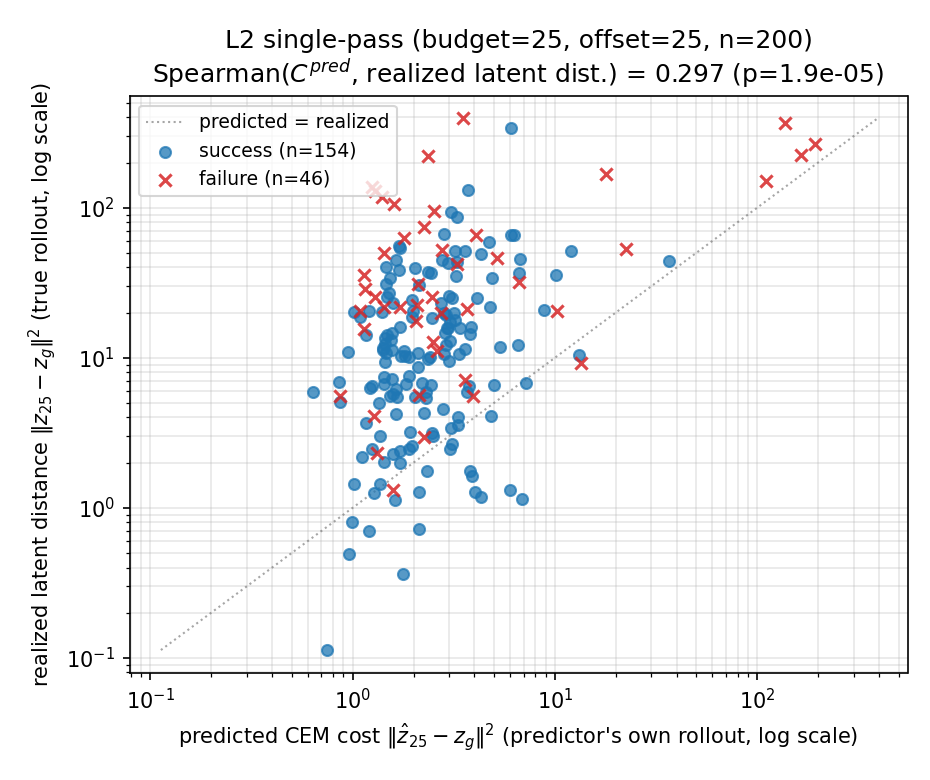
\includegraphics[width=0.72\textwidth]{fig_l2_single_pass_predicted_vs_realized}
  \caption{Single-pass ($n=200$, offset 25, budget 25) L2 CEM: predicted latent cost
  $\|\hat\z_{25}-\z_g\|^2$ (from the predictor's own imagined rollout) vs.\ realized latent
  distance $\|\z_{25}-\z_g\|^2$ (true final frame, re-encoded), both log scale, colored by
  success/failure. Dotted line: $C^{\mathrm{pred}}=C^{\mathrm{real}}$; points above it are
  where the predictor was optimistic.}
  \label{fig:l2-single-pass}
\end{figure}

\subsection{Graph vs.\ L2 candidate ranking across horizon, and why L2 loses (2026-09-21)}
\label{sec:graph-vs-l2-ranking}
\emph{Scripts: \texttt{scripts/viability\_inversion\_audit.py} (offset 10, new; offsets 25/50
reuse the existing Experiment-2 audit) and \texttt{scripts/graph\_candidate\_ranking\_diag.py}
(new). Answers the open question of whether the graph is only a long-horizon tool.}

\paragraph{Setup.} The Experiment-2 privileged-oracle audit (the viability-critic line's
mechanism, \texttt{scripts/viability\_inversion\_audit.py}) fixes 50 (start, goal) problems per offset and, for each, a pool of $K=32$
candidate 25-step action sequences; it stores every candidate's LeWM-predicted terminal
latent $z_{\mathrm{pred}}$, the truly-executed terminal latent $z_{\mathrm{true}}$ (real
physics, same actions), the goal latent $z_g$, and the oracle's true minimum recovery time
$T$ from the executed endpoint. \texttt{graph\_candidate\_ranking\_diag.py} scores every
candidate with four costs -- LeWM's own $\|z-z_g\|^2$ (\textbf{l2}), direct TDR distance with
no graph (\textbf{tdr}), the pure graph route distance (\textbf{geo}), and
$\min(\mathrm{tdr},\mathrm{geo})$ (\textbf{ctg}, the cost \textbf{ctg}/\textbf{subgoal\_tdr}
actually use) -- against $z_{\mathrm{pred}}$ (what the planner sees at decision time) and
separately against $z_{\mathrm{true}}$ (removing predictor error), and reports the mean
per-task Spearman correlation with $T$ (95\% task-bootstrap CI), matching
\texttt{viability\_metric\_vs\_dynamics.py}'s existing convention -- offsets 25/50's
$z_{\mathrm{pred}}$ column reproduces the already-published L2 numbers (0.719/0.356 vs.\
main.tex's 0.72/0.36) as a validation check.

\begin{table}[H]
\centering\small
\caption{Mean per-task Spearman(cost, oracle recovery time $T$), 95\% task-bootstrap CI,
$n=50$ tasks $\times$ 32 candidates. Deployed setting: cost computed on the predictor's own
imagined endpoint $z_{\mathrm{pred}}$, exactly what CEM sees.}
\label{tab:graph-vs-l2-zpred}
\begin{tabular}{lrrrr}
\toprule
offset & l2 & tdr (no graph) & geo (pure graph) & ctg $=\min$(tdr, geo) \\
\midrule
10 & 0.183 [0.09, 0.27] & 0.343 [0.26, 0.42] & \textbf{0.363} [0.28, 0.44] & 0.343 [0.26, 0.42] \\
25 & 0.719 [0.69, 0.75] & \textbf{0.731} [0.69, 0.77] & 0.710 [0.67, 0.75] & \textbf{0.731} [0.69, 0.77] \\
50 & 0.356 [0.25, 0.46] & 0.664 [0.61, 0.71] & \textbf{0.672} [0.62, 0.72] & 0.664 [0.61, 0.71] \\
\bottomrule
\end{tabular}
\end{table}

\paragraph{L2 is not the best candidate-ranker anywhere in this sweep.} The original
hypothesis motivating this check was that L2 should rank candidates best at short range and
the graph should overtake it only at long range. The data does not show that crossover: L2
is worst at offset 10, roughly tied with the graph at 25 (overlapping CIs), and clearly worst
at 50. There is no offset here where L2 wins outright. Offset 10 needs one important caveat,
however: the candidate pool is always a fixed 25-step rollout
(\texttt{HORIZON}$\times$\texttt{SKIP} in \texttt{planning\_cost\_gate.py}), independent of
the audit's goal offset, so at offset 10 every candidate overshoots a goal that is only 10
real steps away by construction -- this is not a clean test of ``short planning horizon,'' and
offset 10's very low numbers should be read with that in mind.

\paragraph{Decomposing the offset-50 gap: predictor error vs.\ metric quality.} Rerunning the
same four costs on $z_{\mathrm{true}}$ (the actually-executed endpoint, so predictor rollout
error is removed) separates two different failure modes that both make L2 look bad at
$z_{\mathrm{pred}}$:

\begin{table}[H]
\centering\small
\caption{Same metric, scored on the true executed endpoint $z_{\mathrm{true}}$ instead of the
predicted one -- isolates the graph's advantage that survives \emph{even with a perfect
predictor}, versus the part that is really about robustness to predictor error.}
\label{tab:graph-vs-l2-ztrue}
\begin{tabular}{lrrrrr}
\toprule
offset & l2 ($z_{\mathrm{pred}}$) & l2 ($z_{\mathrm{true}}$) & ctg ($z_{\mathrm{pred}}$) & ctg ($z_{\mathrm{true}}$) & gap closed by true endpoint \\
\midrule
10 & 0.183 & 0.835 & 0.343 & 0.829 & l2: +0.652; ctg: +0.486 -- l2 catches up \\
25 & 0.719 & 0.809 & 0.731 & 0.833 & l2: +0.090; ctg: +0.102 -- both improve equally \\
50 & 0.356 & 0.454 & 0.664 & 0.734 & l2: +0.098; ctg: +0.070 -- gap persists \\
\bottomrule
\end{tabular}
\end{table}

\textbf{At offset 10, the gap is almost entirely predictor error, not metric quality.} Given
the true endpoint, L2 and the graph are statistically indistinguishable (0.835 vs.\ 0.829,
L2 marginally \emph{ahead}). The z\_pred gap (0.183 vs.\ 0.343) all but disappears once the
predictor's rollout error is removed -- consistent with the horizon-mismatch caveat above: L2
is simply more sensitive to the specific noise that a mismatched 25-step rollout injects at
this offset, not intrinsically a worse metric once given an accurate endpoint. At offset 25
the two metrics improve by almost the same amount with the true endpoint (+0.090 vs.\
+0.102), so neither predictor error nor metric quality dominates -- consistent with the two
metrics being statistically tied at this offset already.

\textbf{At offset 50, the story flips: the gap survives a perfect predictor.} Handing L2 the
ground-truth endpoint only recovers 0.098 of Spearman (0.356 $\to$ 0.454); the graph, scored
on the noisier predicted endpoint, already exceeds L2's \emph{true-endpoint ceiling}
(0.664 $>$ 0.454). This means raw latent L2 distance is an intrinsically weak proxy for
``how many actions until success'' at $\sim$50-step range, independent of how well LeWM's
predictor rolls forward. This is consistent with the mechanism the Findings log's Phase 1
analysis (below) already identified behaviourally (L2's closest approach to the goal is 32\,px but it
drifts back out to 76\,px by the time the episode ends: it gets near, then the block
specifically -- not the agent -- fails to stay converged) and gives it a metric-level
explanation: raw latent L2 pools every state dimension into one Euclidean norm with no notion
of how many actions each dimension actually costs to fix, so a state where the agent already
sits on target but the block is still far away can score as ``close'' even though the
remaining task is not nearly done. TDR is trained on an expectile-TD loss over real transition
counts (Setup, above), so $\psi$ warps the latent specifically so that distance
\emph{is} action-count, weighting each dimension by how expensive it actually is to move, not
by how large it looks in the raw embedding. That training signal is exactly what raw L2 lacks,
and it is why the graph's advantage grows with horizon (more opportunity for the L2-vs-actions
mismatch to compound) rather than shrinking.

\subsection{Live CEM trace: does OUR rank its own elites better than L2? (2026-09-21)}
\label{sec:cem-trace-audit}
\emph{Script: \texttt{scripts/gas\_mpc\_cem\_trace\_audit.py}. Unlike
\cref{sec:graph-vs-l2-ranking}'s fixed diagnostic pool (32 candidates spanning near-expert to
random), this scores the actual 300-candidate population OUR's own live CEM solver samples
and the actual top-30 elites it selects.}

\paragraph{Setup.} For 25 held-out \texttt{task200u} tasks per protocol (\texttt{same25},
\texttt{same50}, CEM seed 0), OUR (\texttt{subgoal\_tdr} + phase-8 final switch + ET critic,
$\beta=1$ -- \cref{sec:phase8} configuration B) runs its normal CEM solver (300 samples, 30
iterations, top-30 elites) for only the \emph{first} plan call (no replanning, no env
execution beyond the CEM optimisation itself). A callback on the solver captures, at
iterations 1, 10, and 20, the 30 elite candidates OUR's own cost selects; each elite's
25-step action sequence is then executed for real in the simulator from the task's true
start state, and the privileged real-physics oracle (\cref{sec:graph-vs-l2-ranking}'s
mechanism, same settings) is run from each elite's true endpoint to the goal. This gives an
oracle recovery-time ranking of the exact elites OUR's optimisation actually kept, so OUR's
cost and LeWM's own z-space L2 (computed for free on the same predicted rollout every
iteration, since both criteria see identical predicted latents -- only their formula differs)
can both be scored against it.

\begin{table}[H]
\centering\small
\caption{Spearman(cost, oracle recovery time) and mean $|{\rm rank(cost)}-{\rm rank}(T)|$
(0 = perfect agreement, $\approx$10 = uncorrelated for $n=30$), over OUR's own 30 elite
candidates, 25 tasks, 95\% task-bootstrap CI where shown.}
\label{tab:cem-trace-audit}
\begin{tabular}{llrrrr}
\toprule
protocol & iteration & $\rho$(OUR) & $\rho$(L2) & mismatch(OUR) & mismatch(L2) \\
\midrule
same25 & 1  & 0.327 [0.25, 0.40]   & 0.396 [0.29, 0.49]   & 7.68 & 7.09 \\
same25 & 10 & 0.168 [0.07, 0.26]   & 0.184 [0.06, 0.30]   & 8.23 & 8.19 \\
same25 & 20 & 0.049 [$-$0.05, 0.15] & 0.106 [$-$0.02, 0.23] & 8.25 & 8.07 \\
same50 & 1  & 0.203 [0.10, 0.30]   & 0.086 [$-$0.06, 0.23] & 8.37 & 9.03 \\
same50 & 10 & 0.150 [0.06, 0.24]   & 0.190 [0.08, 0.30]   & 8.30 & 8.02 \\
same50 & 20 & 0.100 [0.03, 0.17]   & 0.089 [$-$0.04, 0.22] & 8.53 & 8.59 \\
\bottomrule
\end{tabular}
\end{table}

\paragraph{Within its own elites, OUR does not rank better than L2.} Every row's confidence
intervals overlap heavily; the sign of the (small) gap flips between protocols and iterations
(L2 nominally ahead at every same25 iteration, OUR ahead at same50 iterations 1 and 20). This
is a real contrast with \cref{tab:graph-vs-l2-zpred}, where the graph clearly beat L2 at
offset 50 (0.664 vs.\ 0.356) on a wide, fixed candidate pool. Both correlations here are also
much weaker than that table's (0.05--0.4 vs.\ 0.6--0.7) and decay from iteration 1 to 20 for
\emph{both} costs, consistent with a restricted-range effect: by iteration 20 the top-30 have
already converged into a narrow cluster around the running optimum, leaving little spread for
either metric to rank.

\paragraph{Reading.} The graph's advantage over L2 documented earlier in this project is not
``ranks an already-converged elite set more precisely.'' It is upstream of that: which
candidates survive each iteration's elite cut shapes where the population's mean moves over
the following iterations, and \cref{sec:graph-vs-l2-ranking}'s wide-pool result shows the
graph is a better cost \emph{to decide that} when the candidates span a broad range (near
expert to random). Once CEM has already narrowed to a tight elite cluster, however, neither
cost discriminates much further within it -- the mechanism's payoff is in steering the search
trajectory over the full 30 iterations, not in a sharper final ranking at any single
iteration. This is consistent with, and gives a mechanistic account under, the standing
closed-loop finding that OUR's benefit shows up over full episodes at offset 50+ rather than
as a single-solve ranking improvement.

\section{Findings log}
% Entries are appended as runs finish; each states what was run, what happened, the
% diagnosis, and the next decision.

\subsection{Phase 1 (2026-09-14/15): the screen, seed 0, 50 pairs per protocol}
\paragraph{What ran.} Every objective in the seed-0 screen tables in \texttt{legacy\_results.tex} on the same three pair
sets (same-episode offsets 25 and 50, cross-episode), L2 also at offset 100. L2 and the
graph-free TDR cost ran on the laptop (RTX 3050 Ti); the rest on Ada (3$\times$1080 Ti, job
2696687). Lookahead 13.7 TDR units is the calibrated TDR distance of a 25-step gap, i.e.
the subgoal is placed one CEM horizon ahead.

\paragraph{Offset 25: no regression, no gain.} 78--88\% for everything; L2 itself is 88\%.
The only notable drop is \textbf{dir} (78\%), the direction-only cost.

\paragraph{Offset 50: the graph helps, and it is the graph, not just the metric.}
L2 40\% $\to$ TDR 48\% $\to$ ctg 50\% $\to$ subgoal\_tdr 58\%. The median \emph{final}
agent+block error tells the mechanism: L2's closest approach is 32\,px but it ends at 76\,px
(it gets near, then the block drifts away); subgoal\_tdr's closest approach is 19\,px and it
ends at 19\,px. With a subgoal one horizon ahead the planner keeps converging instead of
wandering once L2's ranking goes flat. \textbf{path} (5 waypoints) does not help (42\%): the
waypoint spacing assumes TDR units track env steps block by block, and the intermediate
latents are the predictor's least reliable outputs. \textbf{dir} collapses to 26\%: an
unbounded progress term with no distance in it overshoots the node.

\paragraph{Cross-episode: nothing moves.} L2 8\%, TDR 10\%, ctg 10\%, subgoal\_tdr 10\%,
path 6\% (4--5 successes out of 50 in every case; the pooled 5-seed L2 baseline is 10.8\%).
The per-pair diagnostic (the \texttt{tab:pair-diag-cross-s0} table in \texttt{legacy\_results.tex}) is the important number: by the
graph's own geodesic, the 50 cross-episode pairs are \textbf{45--86 env steps apart (median
66, max 119)}---every one of them inside the 250-step budget, none of them beyond the
horizon the graph objective handles at offset 50. The objective knows a data-supported route;
CEM does not execute it. The successes are still the pairs whose block starts near its goal
pose (2/8 ``block near'' vs 3/42 ``block far'' for subgoal\_tdr).

\paragraph{Diagnosis.} Two facts together---(i) the graph objective wins at offset 50 by
keeping the planner converging near the goal, (ii) it changes nothing on cross-episode pairs
that the same graph rates as 45--120 steps away---say the cross-episode bottleneck is the
low-level executor, not the objective: 25 actions chosen open-loop from a zero-mean Gaussian
proposal, replanned every 25 steps, cannot string together the block pushes that a 66-step
expert route needs. That matches the earlier failure analysis of L2 (agent reaches its own
target, block displaced but never converging).

\paragraph{Decision.} Phase 2 runs both branches: the executor branch---replan every 5--10
steps (\texttt{receding} 1/2), warm-start CEM's mean from the logged 25-action block of the
dataset frame that starts nearest the current state and lands nearest the chosen node
(\texttt{retrieval}), and add the viability critic as a standardised feasibility term
(\texttt{critic\_beta}); (A) confirm the offset-50 gain on seeds 1--2, check cross on seeds
1--2, sweep $\Htd\in\{12,16\}$ and lookahead $\{8,20\}$, and map offset 100.

\subsection{Phase 2 (2026-09-15, Ada): both branches}
\paragraph{Branch A -- confirmation and sweeps.} The offset-50 gain is real across seeds:
\textbf{subgoal\_tdr} 58 / 52 / 56\% on seeds 0 / 1 / 2 against L2 40 / 28 / 48\% (mean
$+16.7$ points, all three seeds positive, the same 50 pairs per seed for both rows). It also
carries to offset 100 (30\% vs.\ L2 22\%; tdr and ctg 28\%). The sweeps are flat-to-mild:
lookahead 8 / 13.7 / 20 TDR units gives 50 / 58 / 56\%; $\Htd=12$ (5,632 nodes) gives 64\% at
offset 50 but 8\% on cross-episode, $\Htd=16$ (2,041 nodes) 50\%. The z-space variant
\textbf{subgoal} (LeWM's own L2 to the node's medoid frame) is 56\% at offset 50 and 16\% on
cross-episode, so the metric used for the last 25 steps barely matters; \emph{where} the
subgoal sits is what matters. Cross-episode with the plain subgoal objective stays at the
floor on a second seed too (12\% on seed 1).

\paragraph{Executor branch.} Three interventions on cross-episode
(seed 0, L2 8\%, plain subgoal\_tdr 10\%):
\begin{itemize}[nosep]
  \item \textbf{Replan every 10 steps} (\texttt{receding} 2): 18\% on cross, but 36\% at
        offset 50 (down from 58). Closed-loop tracking helps a little on the hard pairs and
        hurts the easy ones---the Alg.-1 node re-selection every 10 steps flips targets
        before the 25-step plan has done its work.
  \item \textbf{Retrieval warm-start} (CEM mean = the logged 25-action block of the dataset
        frame starting nearest $\psiT(\z_0)$ and landing nearest the node): 24\% on cross
        (12/50), 54\% at offset 50 (no change). Its wins are early (hits at steps 22--71),
        i.e.\ it executes the first pushes well, but the final error is unchanged (median
        129\,px)---it does not stop the drift.
  \item \textbf{Viability critic} (cost = standardised subgoal cost $+$ standardised
        $-\log V(\hat\z_5, \z_g, h_{\mathrm{rem}})$, the critic from the viability line,
        median/IQR over each CEM population): \textbf{26\% on cross (13/50) and 72\% at offset
        50 (36/50)}---the best number on both protocols by a wide margin. Its wins are the
        genuinely far pairs (10 of the 42 ``block far'' pairs; 9 of the pairs the graph rates
        50--100 steps away, vs.\ 2 for every other objective), its hits spread over the whole
        250-step budget, and its median final error is 59\,px / $9^\circ$ (plain subgoal\_tdr
        125\,px / $19^\circ$, L2 163\,px / $71^\circ$). The critic is what stops the drift.
\end{itemize}

\paragraph{Reading.} The subgoal objective fixes \emph{direction} (it keeps the planner
converging on a data-supported route one horizon at a time) and the critic fixes
\emph{feasibility} (it vetoes endpoints from which the goal is no longer reachable in the
remaining budget). Neither alone moves cross-episode; together they triple it. Retrieval is
a weaker, complementary lever (better first pushes, no drift control).

\paragraph{Decision.} Phase 3: the critic-alone control (L2 $+$ critic, to separate the
critic's contribution from the composition), critic $+$ retrieval, critic $+$ z-space
subgoal, critic $+$ $\Htd=12$, $\beta\in\{0.5,2\}$, offset 100, and seeds 1--4 of the winner
with matched L2 rows for a pooled 250-pair comparison against the 10.8\% baseline.

\subsection{Phases 3--4 (2026-09-15, Ada): controls, combinations, $\beta$, five seeds}
\paragraph{The pooled result.} The \texttt{tab:gas-mpc-pooled-cross-perseed-n50} table in \texttt{legacy\_results.tex}: over the 250 fixed
cross-episode pairs (5 seeds $\times$ 50), with L2 re-run in the same harness on the same
pairs, \textbf{subgoal\_tdr $+$ critic} reaches \textbf{28.0\% at $\beta=1$ (70/250) and
33.6\% at $\beta=2$ (84/250) against L2's 9.6\% (24/250)} (the original 5-seed L2 run gave
10.8\%). Every seed improves: $\beta=2$ gives 38 / 40 / 26 / 34 / 30\% against L2's
8 / 12 / 10 / 8 / 10\%. This is the first cross-episode number in this project above the
$\sim$10\% floor that every RL arm and every plain planning objective has sat at.

\paragraph{Controls: the composition, not the critic alone.} L2 $+$ critic on the same
seed-0 pairs: 12\% at $\beta=1$, 18\% at $\beta=2$ (vs.\ 26\% and 38\% with the subgoal
objective underneath); at offset 50, L2 $+$ critic is 50\% vs.\ 72\% for the composition.
The critic supplies feasibility, the graph subgoal supplies direction; the critic on its own
still has L2's flat long-range ranking to fight. The z-space subgoal composes just as well
(subgoal $+$ critic: 26\%), so again the node choice matters, not the metric to it.
$\Htd=12$ $+$ critic: 22\% cross, 56\% at offset 50---the coarser graph does not help once
the critic is present.

\paragraph{$\beta$ is the lever, and it is not exhausted.} Seed 0 cross-episode:
$\beta=0.5/1/2/4 \to 14/26/38/44\%$, monotone. At offset 50, $\beta=1$ and $2$ are both
72\%; at offset 100, 58\% and 52\% (L2 22\%). The per-pair diagnostic
(the \texttt{tab:pair-diag-cross-s0} table in \texttt{legacy\_results.tex}) shows where the extra successes come from: at $\beta=4$, 17
of the 42 ``block far'' pairs succeed (L2: 3) and 14 of the pairs the graph rates 50--100
steps away (L2: 2). The median final agent+block error falls from 163\,px (L2) to 59 / 35 /
29\,px at $\beta=1/2/4$, and the median block-angle error from $71^\circ$ to $9$--$14^\circ$:
the critic term is what keeps the block from drifting after the first approach. The cost of
a larger $\beta$ is speed---the median first-hit step rises from 96 ($\beta=1$) to 248
($\beta=4$)---so very large $\beta$ would eventually run into the 250-step budget.

\paragraph{Retrieval on top of the critic.} $\beta=1$ $+$ retrieval warm-start: 44\% on seed
0 (22/50, median final error 26\,px, 7 of the 8 ``block near'' pairs and 15 of 42 far ones),
the joint best with $\beta=4$; at offset 50, 64\% (critic alone 72\%). $\beta=2$ $+$
retrieval: 30\% (below $\beta=2$ alone, 38\%). With one seed these two are within noise of
each other ($\pm$3 pairs), so retrieval's contribution on top of the critic is unresolved;
retrieval without the critic (24\%) and the critic without the subgoal (12--18\%) are both
clearly below the composition.

\paragraph{What did not work.} Faster replanning (\texttt{receding} 1/2) hurts at offset 50
and only slightly helps cross; combined with retrieval it collapses (6\%)---a retrieved
25-step block thrown away after 10 steps is worse than either alone. The direction-only cost
(\textbf{dir}) and the waypoint-tracking cost (\textbf{path}) are below L2 at offset 50.
Lookahead and $\Htd$ are flat within noise.

\paragraph{Where this leaves the question.} GAS-style hierarchy inside latent MPC does two
separable things. (1) The graph subgoal one horizon ahead repairs the mid-range regime
(offset 50: 40 $\to$ 58\% on three seeds; offset 100: 22 $\to$ 30\%) by giving CEM a
target inside the range where its cost still ranks correctly. (2) It does nothing for
arbitrary goals on its own, because the executor---25 open-loop actions from a Gaussian
proposal---cannot carry out a 45--120-step route even when the graph knows one. Adding the
viability critic as a standardised feasibility term is what turns the route into
successes: $9.6 \to 33.6\%$ pooled at $\beta=2$, $44\%$ on seed 0 at $\beta=4$. The next
experiments are the ones this table points at: $\beta\in\{4,8\}$ on all five seeds,
retrieval $+$ $\beta\ge 2$ on all five seeds, and 100 pairs per seed for the finalists so
the $\pm$3-pair noise stops deciding rankings.

\subsection{Phase 5 (2026-09-15, Ada job 2697130): $\beta$ and retrieval on all five seeds}
\paragraph{What ran.} $\beta\in\{4,8\}$ on every seed, $\beta=1$ $+$ retrieval on every
seed, $\beta=4$ $+$ retrieval on seeds 0--2, $\beta=2$ at offsets 50 (seeds 0--1) and 100,
$\beta=4$ at offsets 50 and 100, and a fresh 100-pair cross-episode set (seed 0) for L2,
$\beta=4$, and $\beta=1$ $+$ retrieval.

\paragraph{The seed-0 extras do not survive.} Pooled over 250 pairs
(the \texttt{tab:gas-mpc-pooled-cross-perseed-n50} table in \texttt{legacy\_results.tex}): $\beta=0.5/1/2/4/8 \to$ --/28.0/\textbf{33.6}/27.2/25.6\%.
Seed 0's 44\% at $\beta=4$ was the top of its noise band (its other seeds: 28/18/22/24\%).
$\beta=8$ is clearly past the useful range: on seed 2 it has no success before step 175,
i.e.\ the critic term makes the planner too cautious to move. At offset 50, $\beta=4$ gives
64\% (vs.\ 72\% at $\beta=1$ and $2$) with only 18\% of successes inside 50 steps (40\% at
$\beta=1$); at offset 100, 50\% (vs.\ 58 / 52\%). So $\beta=2$ is the setting: the best
cross-episode number, no cost at offsets 50 or 100.

\paragraph{Retrieval is a wash on top of the critic.} $\beta=1$ $+$ retrieval pooled: 32.4\%
(22/15/11/25/8 successes per seed---the widest spread of any row); $\beta=4$ $+$ retrieval
on three seeds: 30.0\%. Both sit between $\beta=1$ alone (28.0\%) and $\beta=2$ alone
(33.6\%), so warm-starting CEM from logged action blocks neither helps nor hurts once the
critic is present. On the fresh 100-pair set, L2 is 10\%, $\beta=4$ 36\%, $\beta=1$ $+$
retrieval 36\%---consistent with the pooled 50-pair numbers.

\paragraph{Offset 50 is stable across seeds with the critic.} $\beta=2$: 72\% on seeds 0
and 1 (plain subgoal 58 / 52\%, L2 40 / 28\%).

\paragraph{Standing result (superseded by phase 8).} \textbf{subgoal\_tdr $+$ critic, $\beta=2$: 33.6\% over the
250 fixed cross-episode pairs (L2 9.6\% on the same pairs and solver), 72\% at offset 50
(L2 40\%), 52--58\% at offset 100 (L2 22\%).} The remaining knobs (retrieval, $\beta>2$,
replan rate, $\Htd$, lookahead) are exhausted at this pair count; the TE-threshold and
state-regime ($\text{expectile}=0.999$, $\theta_{\mathrm{TE}}=0.99$) checks are queued as
phases 6--7.

\subsection{Phase 8 (2026-09-16, Ada job 2698367): closing the short-range gap and the $\beta$ dependence}
\label{sec:phase8}
\paragraph{Diagnosis.} Three things explain why L2 wins at offset 25 while the critic composition
wins everywhere else. (i) The critic is a feasibility classifier: at offset 25 the CEM population is
almost entirely feasible, $V$ saturates and $-\log V$ carries only calibration noise; the audit
confirms it ranks predictor endpoints worse than L2 exactly there (Spearman vs.\ oracle 0.60 at
$h=25$ vs.\ L2's 0.72; 0.70 vs.\ 0.36 at offset 50). The $\beta$ sweep at same25 (87 $\to$ 82 $\to$
79 $\to$ 75 $\to$ 68) is the planner sliding toward pure-$V$ behaviour, which the viability line
measured at 66\% closed-loop. (ii) Per-population median/IQR standardisation forces each term to a
fixed vote share whatever it knows: a saturated critic term is stretched to unit spread and added
with weight $\beta$, so $\beta$ alone decides the regime. (iii) With the final-goal switch at
$\Htd=8$ units ($\approx$12 steps) the first same25 solve still targets a cluster medoid whose
radius ($\Htd/2\approx 6$ steps) is comparable to the success tolerance; neither term has L2's
resolution at the goal (subgoal\_tdr alone already loses 91 $\to$ 87). Feasibility also has no
progress gradient (median first-hit step 96 $\to$ 248 as $\beta$ goes 1 $\to$ 4).

\paragraph{What ran.} Five configurations on the fixed task set, 50 tasks, seeds 0--2, every
protocol (\texttt{scripts/ada\_gas\_mpc\_phase8.sh}):
\begin{itemize}[nosep]
  \item \textbf{A} subgoal\_tdr with the final-goal switch at one lookahead
        (\texttt{final\_thresh}=13.7 units $\approx$ 25 steps) and LeWM's z-space L2 as the
        final-phase cost (\texttt{final\_metric=l2}): the method reduces to L2 wherever L2 is
        best.
  \item \textbf{OUR} A $+$ critic with a budget-capped expected hitting time,
        $\mathrm{ET}=5\sum_{h\le h_{\mathrm{rem}}}(1-V(\hat\z_5,\z_g,h))$ in env steps
        (\texttt{critic\_cost=et}): ranks feasible endpoints by how soon they arrive, infeasible
        ones at the cap. Standardised composition, $\beta=1$; \textbf{E} the same at $\beta=2$.
  \item \textbf{C} A $+$ ET with both terms in env steps and no standardisation
        (\texttt{compose=steps}): the base distance is converted through the empirical
        median-distance-by-step-gap table (\texttt{outputs/gas\_mpc/gap\_calib\_s\{seed\}.json},
        TDR units and z-space L2, 12 gaps from 1 to 50), cost $=$ steps-to-subgoal $+$ ET. A
        saturated critic then contributes near-zero spread by itself; no $\beta$.
  \item \textbf{D} A $+$ hard feasibility filter (\texttt{critic\_filter}=0.5): rank by the base
        cost among candidates with $V(\hat\z_5,\z_g,h_{\mathrm{rem}})\ge 0.5$, by $V$ alone if
        none pass. The ``veto'' made literal; one calibrated threshold, no weight.
\end{itemize}
\paragraph{Results (seeds 0--2, 50 tasks; \cref{tab:gas-mpc-subgoal_tdr-crit-task200-n50}).}
Every row below is on the same 150 (task, seed) pairs; ``old $\beta$'' rows are the phase 3--5
configurations restricted to the same three seeds.
\begin{center}\small
\begin{tabular}{lrrrr}
\toprule
configuration & same-ep 25 & same-ep 50 & same-ep 100 & cross-ep \\
\midrule
L2 & 89.3 & 50.7 & 12.0 & 12.7 \\
old subgoal\_tdr & 88.0 & 58.7 & 20.0 & 17.3 \\
old $\beta=1$ / $\beta=2$ ($-\log V$, std) & 81.3 / 78.0 & 62.7 / 59.3 & 41.3 / 40.0 & 29.3 / 33.3 \\
\midrule
A: final switch @13.7 + final L2 & 90.0 & 62.0 & 24.7 & 19.3 \\
OUR: A + ET, std, $\beta=1$ & \textbf{92.0} & \textbf{66.7} & \textbf{47.3} & \textbf{43.3} \\
E: A + ET, std, $\beta=2$ & 90.0 & 65.3 & 40.0 & 38.0 \\
C: A + ET, steps (no std, no $\beta$) & 90.0 & 58.7 & 38.7 & 31.3 \\
D: A + filter $\tau=0.5$ (no $\beta$) & 89.3 & \textbf{66.7} & 44.0 & 33.3 \\
\bottomrule
\end{tabular}
\end{center}
\begin{itemize}[nosep]
  \item \textbf{(a) is closed by the final-phase switch alone.} Every configuration with
        \texttt{final\_thresh}=13.7 and z-space L2 in the final phase is within noise of L2
        at offset 25 (89--92\% vs.\ 89.3\%), including the critic ones that previously lost
        8--13 points; median first-hit step is 24 for all of them, as for L2. The switch also
        lifts the no-critic subgoal objective at every other protocol (58.7 $\to$ 62.0 at
        offset 50, 20 $\to$ 24.7 at 100), i.e.\ the medoid-radius resolution floor was costing
        successes there too.
  \item \textbf{(b) the $\beta$ dependence is gone with the hitting-time cost.} With ET in
        place of $-\log V$, $\beta=1$ is at least as good as $\beta=2$ on every protocol
        (92/66.7/47.3/43.3 vs.\ 90/65.3/40/38); under $-\log V$ the two traded places between
        same25 and cross. One setting, OUR, is now the best or tied-best row on all four
        protocols, and it is the best cross-episode number in the project on these seeds
        (43.3\% vs.\ 33.3\% for the previous $\beta=2$ standing result; final agent+block
        error 26\,px / $9^\circ$ vs.\ 40\,px / $10^\circ$; median first hit 95 vs.\ 188 steps).
        ET keeps a progress gradient among feasible endpoints, which is what $-\log V$ lacked.
  \item \textbf{Same units without standardisation (C) works but is the weakest critic
        variant.} It matches L2 at offset 25 and beats the old $\beta$ rows at offset 100 and
        cross only marginally (38.7 / 31.3). Its final errors (53\,px at offset 100, 99\,px on
        cross) say the subgoal term dominates the sum: the calibrated conversion puts a residual
        of a few TDR units at 5--10 ``steps'', comparable to the whole ET range, so the critic's
        veto is diluted exactly on the far pairs. The per-population standardisation, whatever
        its faults at short range, is what gives the critic a full vote at long range; the
        short-range fault is fixed by the switch, not by the composition.
  \item \textbf{The hard filter (D) is a credible $\beta$-free alternative}: 89.3 / 66.7 /
        44.0 / 33.3 with one threshold, tied-best at offset 50, and its statistics show the
        veto doing the intended work (67\% of candidates pass at offset 25 and the fallback
        to $V$-ranking fires on 3\% of solves; 39--41\% pass at offset 100 / cross with the
        fallback on 35--38\% of solves). It trails OUR by 10 points on cross because a
        threshold discards the ranking information among infeasible candidates that ET keeps.
\end{itemize}

\paragraph{Seeds 3--4 for A, OUR, C (same day, two processes per GPU).} Five-seed means
(250 (task, seed) pairs per protocol; per-seed values in the appendix tables):
\begin{center}\small
\begin{tabular}{lrrrr}
\toprule
configuration & same-ep 25 & same-ep 50 & same-ep 100 & cross-ep \\
\midrule
L2 & 91.2 & 48.4 & 11.2 & 10.4 \\
old $\beta=1$ / $\beta=2$ ($-\log V$, std) & 78.8 / 74.8 & 62.4 / 57.2 & 41.6 / 41.6 & 30.8 / 34.4 \\
A: final switch @13.7 + final L2 & 90.8 & 61.2 & 28.8 & 19.6 \\
OUR: A + ET, std, $\beta=1$ & 90.8 & \textbf{64.4} & \textbf{50.4} & \textbf{44.4} \\
C: A + ET, steps (no std, no $\beta$) & 90.0 & 62.0 & 36.0 & 32.0 \\
\bottomrule
\end{tabular}
\end{center}
The two new seeds move nothing qualitatively and strengthen OUR: its cross-episode
per-seed values are 48 / 40 / 42 / 42 / 50 (old $\beta=2$: 32 / 30 / 38 / 32 / 40; L2:
12 / 16 / 10 / 8 / 6), so every seed is 10--18 points above the previous standing result
and OUR is the first configuration to clear 40\% on every cross-episode seed. Offset 100 is
44--57 across seeds (old $\beta$ rows 36--48). At offset 25 OUR is 88--96 against L2's 86--94,
the same band. C stays the weakest critic variant (32.0 cross, 36.0 at offset 100).

\paragraph{Standing result.} \textbf{subgoal\_tdr with the final-goal switch at one lookahead,
z-space L2 in the final phase, and the budget-capped expected-hitting-time critic term at
$\beta=1$ (OUR): 90.8 / 64.4 / 50.4 / 44.4\% at offsets 25 / 50 / 100 / cross over
five seeds, against L2's 91.2 / 48.4 / 11.2 / 10.4 on the same 250 pairs per protocol.}
Remaining checks: $\beta=0.5$ under ET, seeds 3--4 for D and E, and the filter (D) at
$\tau\in\{0.3,0.7\}$ before it is dropped.

\paragraph{Two processes per GPU.} The seed 3--4 cross-episode runs were the first to share
GPUs (two evals per 1080\,Ti). Per-run wall time went from 13.7 / 14.9 / 15.8 min (A / OUR / C,
one process per GPU, seeds 0--2) to 25.5 / 25.5 / 27.1 min, i.e.\ $1.7$--$1.9\times$ slower per
process for $2\times$ the processes: a throughput gain of only 5--20\%. The CEM loop keeps a
1080\,Ti near 100\% on its own, so there is little idle capacity to fill. (A first attempt
had pinned all six processes to GPU~0 through a shell bug and ran $5$--$6\times$ slower; those
runs were discarded and repeated.)


\section{Reacher (dm\_control, \texttt{qpos\_match})}
\label{sec:reacher}
\emph{Second environment for the two headline objectives: L2 and the phase-8 winner OUR.
Pipeline: \texttt{scripts/ada\_gas\_mpc\_reacher.sh} (one resumable script: dataset staging,
encoding, per-seed TDR / graph / critic training with one process per GPU, a render-consistency
guard, then the evaluation sweep with one process per GPU). Results table:
\texttt{results\_table\_reacher.tex}, regenerated by \texttt{GAS\_MPC\_ENV=reacher python
scripts/gas\_mpc\_report.py}.}

\paragraph{Data and task.} \texttt{quentinll/lewm-reacher}: 10,000 episodes of exactly 201
frames (2.01M frames, 224$\times$224), columns \texttt{qpos}/\texttt{qvel} (2 joints each)
rather than a \texttt{state} column; the state vector used everywhere below is qpos$|$qvel.
The frozen LeWM Reacher checkpoint has the same latent (192-d CLS) and action-block
convention (5 actions $\times$ 2 dims $=$ 10) as Push-T. Success is the env's own
\texttt{qpos\_match} termination: every joint within 0.05\,rad of the target qpos, as a
\emph{raw} difference (no angle wrap) -- the shoulder is an unlimited hinge and the dataset's
shoulder angle is unwrapped over roughly $\pm 8$\,rad, so a goal one full turn away counts as
far, exactly as the env scores it. Protocols as for Push-T (same-episode offsets 25 / 50 / 100
with budget $2K$; cross-episode with budget 200 $=$ the dataset episode length), fixed
200-task sets drawn from the same \texttt{TASK\_SEED}, first 50 used, 5 seeds.

\paragraph{Hyperparameters and what was changed for this environment.}
\begin{itemize}[nosep]
  \item \textbf{Unchanged:} TDR (32-d, expectile 0.99, $\gamma=0.99$, 50k steps), TE
        threshold 0.9, CEM (300 / 30 / top-30, horizon 5 blocks, open-loop 25 steps), critic
        architecture and losses ($h_{\max}=50$, $\delta_{\max}=60$, 5 members, 60k steps,
        Bellman + monotonicity), $\beta=1$, ET cost for OUR.
  \item \textbf{Graph radius and lookahead in env steps, not TDR units.} Push-T's $\Htd=8$ and
        lookahead 13.7 are TDR-unit values that happen to equal $\approx$12 and 25 env steps of
        that TDR. The Reacher TDR has its own scale, so both are read off seed 0's calibrated
        median-distance-by-gap table after TDR training ($\Htd$ = distance at 12 steps,
        lookahead $=$ final-goal switch $=$ distance at 25 steps; \texttt{calib.json}) and
        shared by all seeds (Push-T's per-seed 25-step distances differ by $<3\%$, so one
        table is safe and keeps one method tag per configuration).
  \item \textbf{Critic cross-episode negatives gated in joint space.} Push-T only labels a
        cross-episode pair unreachable when the block poses differ by $\ge 100$\,px. The
        Reacher analogue is the joint-space L2 distance; measured on the data, no 50-step
        window ever moves the joints more than 2.35\,rad (99th percentile; 3.81 max), so
        pairs $\ge 2.5$\,rad apart (about 60\% of random cross pairs, whose median distance is
        3.26\,rad) are safe negatives and closer ones are left unlabelled.
  \item \textbf{Hindsight labels are tight here.} With the 0.05-rad tolerance the logged arm
        essentially never passes within tolerance of a later frame before reaching it (on
        20k random ($t$, $t{+}50$) pairs the first hit is the goal step itself), so the
        hindsight label is $1[h \ge \delta]$ with no behavioural slack -- unlike Push-T's
        loose 20-px / 20$^\circ$ predicate.
\end{itemize}

\paragraph{Calibration and graph.} TDR: Spearman vs.\ the privileged state-distance oracle
0.93, vs.\ the true step gap 0.82 (seed 0). The calibrated median-distance-by-gap table
(\texttt{outputs/gas\_mpc\_reacher/calib.json}) gives $H_{\mathrm{TD}}=3.93$ TDR units at a
12-step gap and lookahead/final-switch $=5.78$ units at 25 steps -- both far smaller than
Push-T's 8 and 13.7, i.e.\ Reacher's TDR is a flatter, less spread-out metric. The graph at
TE$=0.9$ keeps 48\% of frames as nodes ($\approx$530--540 nodes, $\approx$1900 edges, one
connected component) -- roughly 40$\times$ sparser than Push-T's 20.5k-node graph, consistent
with Reacher's 2-DoF state space needing far fewer landmarks to cover.

\paragraph{Critic.} Trained with \texttt{viability\_train.py --env reacher} on the same
architecture as Push-T ($h_{\max}=50$, $\delta_{\max}=60$, 5 members, 60k steps, Bellman +
monotonicity), cross-episode negatives gated at joint-space L2 $\ge 2.5$\,rad (the data never
moves more than 2.35\,rad, p99, in a 50-step window). Final validation: hindsight
AUROC 0.906, ECE 0.010, imagined-rollout AUROC 0.94, monotonicity violation rate 0.4\% --
in the same range as the Push-T critic's own diagnostics.

\paragraph{The live env must render what the encoder was trained on.} The first
evaluation pass on Reacher (2026-09-16/17) gave L2 64.8\% at offset 25, twenty points under the
LeWM paper's 86\% (Fig.~6; PLDM 78, DINO-WM 79, random 10). The cause was not the planner:
\texttt{reacher.h5} was rendered with MuJoCo 3.5/3.6 (March 2026), while the Ada environment
had MuJoCo 3.12.0, which draws the dm\_control floor \emph{without} its checker texture. At the
same (qpos, qvel) the arm is pixel-identical but the mean pixel difference to the stored frame
is 18/255, and the frozen encoder moves the latent by a median of 15.1 units -- about a whole
25-step gap (17.4; 1-step 3.0) and not a constant offset (11.8 remains after removing the mean
shift). With the arm exactly at the goal the live latent still sits 15.4 from the goal latent,
so the terminal-L2 cost never approaches zero; nearest-neighbour state retrieval from live
frames into a dataset-frame bank recovers the joint state within 0.05\,rad only 3\% of the time
(dataset frames: 100\%). Pinning \texttt{mujoco==3.5.0 dm\_control==1.0.37} restores the dataset
look exactly (0.0 mean pixel difference) and L2 at offset 25 to $86.8 \pm 4.8$ (80/84/88/92/90;
$84.0 \pm 2.4$ with the paper's own 10 CEM iterations instead of our 30) -- the paper's number.
The launcher now refuses to evaluate unless three dataset frames re-render to within 4/255 of
the stored pixels. Push-T is unaffected (pygame/pymunk, no MuJoCo): the same check gives a
0.49/255 pixel difference and a 0.67-unit latent shift, below its own 1-step gap of 1.06.
Every Reacher number in this section is from the corrected render; the first pass (L2
64.8/60.0/63.6/17.2, OUR 68.4/68.4/73.2/36.4) is superseded and its files were deleted. Two
protocol differences from the paper remain and are minor: the paper draws Reacher start/goal
pairs from a random-policy dataset (\texttt{dmc/reacher\_random}, not shipped) whereas ours come
from the SAC training set, and it uses 10 CEM iterations on Reacher (30 only on Push-T).

\subsection{Results (2026-09-17, Ada job 2698921, corrected render)}
\paragraph{What ran.} The two headline configurations from the Push-T line, on the fixed
200-task set (first 50 used), seeds 0--4, all four protocols: \textbf{l2} (LeWM's own terminal
latent L2) and \textbf{OUR} (\texttt{subgoal\_tdr} $+$ final-goal switch at one lookahead
(\texttt{final\_thresh}=5.78) $+$ z-space L2 in the final phase $+$ the budget-capped
expected-hitting-time critic term, std composition, $\beta=1$ -- the phase-8 Push-T winner).
The phase-3 composition (``old'': $-\log V$, std, $\beta=1$) was dropped from the default sweep;
under the broken render it sat below L2 on every same-episode protocol, as on Push-T, and has
not been rerun. No $\beta$ sweep and no \textbf{C}/\textbf{D}/\textbf{E} variants have been run
on Reacher. Protocol budgets: same-ep 25/50/100 at $2\times$ the offset (50/100/200 steps);
cross-episode at 200 steps (Reacher's full episode length, vs.\ Push-T's 250). All 40
seed$\times$protocol$\times$config runs completed in 85 minutes with one process per GPU
(the earlier ``two per GPU OOMs'' was every process's $\approx$2\,GB EGL render context landing
on GPU~0 -- dm\_control picks EGL device 0 regardless of \texttt{CUDA\_VISIBLE\_DEVICES}; the
launcher now sets \texttt{MUJOCO\_EGL\_DEVICE\_ID} per slot). Full per-seed detail is in the
regenerated appendix, \texttt{results\_table\_reacher.tex}.

\begin{center}\small
\begin{tabular}{lrrrr}
\toprule
configuration & same-ep 25 & same-ep 50 & same-ep 100 & cross-ep \\
\midrule
l2 & \textbf{86.8} $\pm$ 4.8 & 96.0 $\pm$ 1.4 & 76.0 $\pm$ 1.4 & 24.4 $\pm$ 1.7 \\
OUR (final switch, final L2, ET, $\beta=1$) & 80.8 $\pm$ 5.2 & \textbf{97.6} $\pm$ 2.6 & \textbf{98.0} $\pm$ 0.0 & \textbf{64.0} $\pm$ 2.8 \\
\bottomrule
\end{tabular}
\end{center}

\begin{center}\small
\begin{tabular}{lrrrrrr}
\toprule
configuration & s0 & s1 & s2 & s3 & s4 & pooled \\
\midrule
l2 (same25) & 80 & 84 & 88 & 92 & 90 & 217/250 \\
l2 (same50) & 96 & 96 & 96 & 94 & 98 & 240/250 \\
l2 (same100) & 76 & 74 & 76 & 76 & 78 & 190/250 \\
l2 (cross) & 24 & 26 & 24 & 26 & 22 & 61/250 \\
\midrule
OUR (same25) & 80 & 76 & 88 & 84 & 76 & 202/250 \\
OUR (same50) & 100 & 96 & 98 & 94 & 100 & 244/250 \\
OUR (same100) & 98 & 98 & 98 & 98 & 98 & 245/250 \\
OUR (cross) & 64 & 64 & 60 & 68 & 64 & 160/250 \\
\bottomrule
\end{tabular}
\end{center}

\paragraph{OUR's gain is concentrated where the horizon exceeds one plan.} Per-seed OUR$-$L2:
same25 $0/{-}8/0/{-}8/{-}14$ (OUR loses 6 points pooled, 80.8 vs.\ 86.8 -- the same short-range
picture as Push-T, where OUR and L2 tie at 90.8 vs.\ 91.2), same50 $+4/0/{+}2/0/{+}2$ (tie at
the ceiling, 97.6 vs.\ 96.0), same100 $+22/{+}24/{+}22/{+}22/{+}20$ (every seed; OUR solves 49 of
the 50 tasks in every seed while L2 stays at 76\%), cross $+40/{+}38/{+}36/{+}42/{+}42$ (every
seed; \textbf{2.6$\times$}, 64.0 vs.\ 24.4\% -- 160/250 vs.\ 61/250 hits). Under the broken
render the same comparison read as a uniform $+4$ to $+10$ with $2\times$ on cross-episode;
with frames the encoder recognises, L2 is at the paper's level at short range and the
separation moves entirely to the long-horizon and cross-episode protocols, exactly the
regime the subgoal graph and the hitting-time critic are built for.

\paragraph{L2 on Reacher: strong at one or two plans, then it stalls.} 86.8 / 96.0 at offsets
25 / 50, but 76.0 at offset 100 and 24.4 cross-episode, against Push-T's 91.2 / 48.4 / 11.2 /
10.4. Reacher's 2-DoF joint space keeps the goal ``visible'' to the terminal-L2 cost far longer
than Push-T's block manipulation does, so the baseline degrades slowly rather than collapsing;
the failures at 100 steps and cross-episode are near-misses that stall outside the 0.05-rad
band, which is what the graph's intermediate targets and the critic's progress term fix.

\paragraph{Caveats.} (a) No $\beta$ sweep, retrieval, or the \textbf{C}/\textbf{D}/\textbf{E}
ablations from the Push-T phase-8 study have been run on Reacher; $\beta=1$ is the only value
tested. (b) Cross-episode success on Reacher is an intrinsically harder bar than it looks --
the shoulder joint is unwrapped ($\approx\pm8$\,rad), so a goal a full turn away scores as far
even when the two poses are physically close, which likely caps how high any method's
cross-episode number can go. (c) The short-range loss of OUR (80.8 vs.\ 86.8 at offset 25) is
within one seed's spread but consistent in sign (0 or negative in every seed); the same
final-phase switch that closed this gap on Push-T does not fully close it here, and has not
been tuned for Reacher's TDR scale.

\section{Cube (OGBench, \texttt{swm/OGBCube-v0}, single cube)}
\label{sec:cube}
\emph{Third environment for the two headline objectives, L2 and OUR. Pipeline:
\texttt{scripts/ada\_gas\_mpc\_cube.sh} (one resumable script, cloned from the Reacher one:
dataset download straight onto the compute node's \texttt{/ssd\_scratch}, encoding, per-seed
TDR / graph / critic with one process per GPU, a render-consistency guard, then the evaluation
sweep). Environment hooks: \texttt{CubeMechanics} in \texttt{scripts/common/envs.py}. Results
table: \texttt{results\_table\_cube.tex}, regenerated by \texttt{GAS\_MPC\_ENV=cube python
scripts/gas\_mpc\_report.py}.}

\paragraph{Data and task.} \texttt{quentinll/lewm-cube} (\texttt{cube\_single\_expert}):
10,000 episodes of exactly 201 frames (2.01M frames, 224$\times$224, 102\,GB decompressed --
staged only on the compute node, no \texttt{/share1} copy). A UR5e arm with a gripper moves one
cube to a target position; actions are 5-d (xyz delta, gripper yaw, gripper) in $[-1, 1]$, and
the frozen LeWM Cube checkpoint's action encoder takes 25-d blocks (5 actions $\times$ 5 dims),
the same frame-skip-5 convention as the other environments. The h5 stores the full simulator
state (\texttt{qpos} 21-d, \texttt{qvel} 20-d) plus flattened privileged / proprio columns;
the state vector used by every script below is [block xyz, effector xyz] (6-d, metres), read
from \texttt{privileged\_block\_0\_pos} and \texttt{proprio\_effector\_pos}. Success is the
env's own predicate (\texttt{CubeEnv.\_compute\_successes}, \texttt{terminate\_at\_goal}): the
cube within \textbf{0.04\,m of its target position} -- position only, no orientation, and
the arm's own pose is irrelevant. The evaluator restores a task's start from the dataset
row's \texttt{qpos}/\texttt{qvel} and sets the target from the goal row's block position and
quaternion (\texttt{config/eval/cube.yaml} callables). Protocols as for Push-T and Reacher
(same-episode offsets 25 / 50 / 100 with budget $2K$; cross-episode with budget 200 $=$ the
episode length), fixed 200-task sets from the same \texttt{TASK\_SEED}, first 50 used, 5 seeds.

\paragraph{Hyperparameters and what was changed for this environment.}
\begin{itemize}[nosep]
  \item \textbf{Unchanged:} TDR (32-d, expectile 0.99, $\gamma=0.99$, 50k steps), TE
        threshold 0.9, CEM (300 / 30 / top-30, horizon 5 blocks, open-loop 25 steps), critic
        architecture and losses ($h_{\max}=50$, $\delta_{\max}=60$, 5 members, 60k steps,
        Bellman + monotonicity), $\beta=1$, ET cost for OUR. Nothing was tuned on Cube.
  \item \textbf{Graph radius and lookahead calibrated in env steps}, exactly as on Reacher:
        $\Htd$ = seed 0's median TDR distance at a 12-step gap, lookahead $=$ final-goal
        switch $=$ the distance at 25 steps (\texttt{calib.json}), shared by all seeds.
  \item \textbf{Critic cross-episode negatives gated on block displacement.} The Cube
        analogue of Push-T's 100-px block gate is the block-position L2 in metres. Measured on
        the data, the block moves 0.157\,m (median) / 0.311 (p90) / 0.477 (p99) / 0.612 (max)
        in any 50-step window, so the gate is set automatically to the p99, 0.477\,m; pairs
        whose blocks are farther apart are safe ``unreachable within $h_{\max}$'' negatives,
        closer ones are left unlabelled.
  \item \textbf{The state-distance oracle is only a diagnostic here.} Raw latent L2 has
        Spearman $-0.04$ against z-scored [block, effector] distance (vs.\ 0.83 against the
        true step gap), i.e.\ block-plus-gripper position is not a proxy for latent distance
        on Cube (the arm's joint configuration dominates the image). The TDR's
        \texttt{rho\_oracle} column is therefore uninformative for this environment; nothing
        in training or planning uses it.
\end{itemize}

\paragraph{Calibration, graph, critic.} TDR (seed 0): Spearman vs.\ the true step gap 0.89
(raw L2 0.83); median distance by gap $\{1{:}\,0.8,\ 2{:}\,1.4,\ 5{:}\,3.4,\ 10{:}\,6.4,\
25{:}\,14.3,\ 50{:}\,19.4\}$, giving $\Htd = 7.49$ and lookahead / final switch $= 14.25$ TDR
units -- almost exactly Push-T's 8 and 13.7, unlike Reacher's much flatter 3.9 / 5.8. The
graph at TE$=0.9$ keeps 75\% of frames (1.48M of 1.97M training frames) and clusters them into
15.8--16.2k nodes with 323--338k edges (mean degree 41), one connected component, $\approx$80\,s
to build -- Push-T scale, not Reacher scale. Critics (5 seeds, 60k steps): held-out hindsight
AUROC 0.990--0.991, ECE 0.006--0.009, imagined-rollout AUROC 0.983--0.995, monotonicity
violation rate 0.4--0.8\%, Bellman residual 0.033--0.037, mean $V$ on gated cross-episode
negatives $\le 0.01$ -- the tightest critic diagnostics of the three environments (Cube's
hindsight labels are nearly slack-free: the block only moves during the carry segment).

\paragraph{Render check.} Following the Reacher lesson, the eval stage first restores three
dataset rows into the live env and compares the render to the stored frame
(\texttt{scripts/gas\_mpc\_cube\_render\_check.py}). With \texttt{mujoco==3.5.0} and
\texttt{ogbench==1.2.1} the mean pixel difference is 0.0 / 0.08 / 0.2 (of 255) and the live
info state equals the h5 state to the millimetre, so the encoder sees exactly the frames it
was trained on. (Practical note: \texttt{ogbench} must be pip-installed from the compute
node; the venv's \texttt{/usr/bin/python3} is 3.10 there but 3.6 on the login node.)

\subsection{Results (2026-09-18, Ada job 2699936)}
\paragraph{What ran.} \textbf{l2} and \textbf{OUR} (\texttt{subgoal\_tdr} $+$ final-goal switch at
one lookahead (\texttt{final\_thresh}=14.25) $+$ z-space L2 in the final phase $+$ the
budget-capped expected-hitting-time critic term, std composition, $\beta=1$), fixed 200-task
sets (first 50 used), seeds 0--4, four protocols; 40 runs in 110 minutes with one process per
GPU. No $\beta$ sweep, retrieval, or \textbf{C}/\textbf{D}/\textbf{E} variants. Full per-seed
detail in \texttt{results\_table\_cube.tex}.

\begin{center}\small
\begin{tabular}{lrrrr}
\toprule
configuration & same-ep 25 & same-ep 50 & same-ep 100 & cross-ep \\
\midrule
l2 & 56.8 $\pm$ 3.2 & 50.8 $\pm$ 1.6 & 62.0 $\pm$ 2.2 & 12.8 $\pm$ 2.7 \\
OUR (final switch, final L2, ET, $\beta=1$) & \textbf{66.8} $\pm$ 5.2 & \textbf{56.4} $\pm$ 4.6 & \textbf{70.4} $\pm$ 0.8 & \textbf{37.6} $\pm$ 4.3 \\
\bottomrule
\end{tabular}
\end{center}

\begin{center}\small
\begin{tabular}{lrrrrrrr}
\toprule
configuration & s0 & s1 & s2 & s3 & s4 & pooled & solved $\ge$1 / all \\
\midrule
l2 (same25) & 54 & 52 & 58 & 60 & 60 & 142/250 & 36 / 19 \\
l2 (same50) & 50 & 50 & 50 & 50 & 54 & 127/250 & 31 / 19 \\
l2 (same100) & 62 & 60 & 66 & 60 & 62 & 155/250 & 37 / 27 \\
l2 (cross) & 16 & 8 & 12 & 14 & 14 & 32/250 & 11 / 4 \\
\midrule
OUR (same25) & 68 & 68 & 74 & 66 & 58 & 167/250 & 42 / 24 \\
OUR (same50) & 52 & 58 & 50 & 62 & 60 & 141/250 & 34 / 20 \\
OUR (same100) & 70 & 70 & 72 & 70 & 70 & 176/250 & 40 / 31 \\
OUR (cross) & 34 & 44 & 40 & 38 & 32 & 94/250 & 29 / 9 \\
\bottomrule
\end{tabular}
\end{center}

\paragraph{OUR beats L2 everywhere, including short range.} Per-seed OUR$-$L2: same25
$+14/{+}16/{+}16/{+}6/{-}2$, same50 $+2/{+}8/0/{+}12/{+}6$, same100 $+8/{+}10/{+}6/{+}10/{+}8$
(every seed), cross $+18/{+}36/{+}28/{+}24/{+}18$ (every seed; \textbf{2.9$\times$}, 37.6 vs.\
12.8\%, 94/250 vs.\ 32/250 hits). Nineteen of the twenty seed$\times$protocol cells favour OUR;
the one exception is a 50--50 tie (same50, seed 2). The cross-episode ratio matches Push-T
(10.4 $\to$ 44.4, $4.3\times$) and Reacher (24.4 $\to$ 64.0, $2.6\times$). Unlike both, OUR also
wins at offset 25 ($+10$ pooled): on Cube even one plan benefits from the subgoal, because the
terminal-L2 cost from a frame where the block has not moved yet is dominated by the arm, not
the block (see the oracle diagnostic above), so L2 alone drifts the arm toward the goal
\emph{image} rather than the goal \emph{block}.

\paragraph{A large share of the tasks are solved at $t=0$.} Cube's predicate ignores the arm
and the block is stationary for most of an episode (it moves only while carried), so many
goal frames have the block exactly where it already is. Tasks whose block starts inside the
4\,cm tolerance: same25 22\%, same50 16\%, same100 \textbf{44\%}, cross 6\%; every such task
succeeds at the first step for either method, and the first-hit histograms confirm it (24\% /
16\% / 44\% / 6\% of hits at step 1). This is why same100 $\ge$ same25 for both methods -- at
a 100-step offset the goal frame is often the block sitting at its final position after the
carry ended. On the remaining tasks, where the block must actually be moved:

\begin{center}\small
\begin{tabular}{lrrrr}
\toprule
block starts $>4$\,cm away & same25 ($n{=}39$) & same50 (42) & same100 (28) & cross (47) \\
\midrule
l2 & 44.6 & 41.4 & 32.1 & 7.2 \\
OUR & \textbf{57.4} & \textbf{48.1} & \textbf{47.1} & \textbf{33.6} \\
\bottomrule
\end{tabular}
\end{center}

\noindent The ordering and the cross-episode gap are unchanged; the absolute numbers are the
ones to compare with a manipulation baseline. The headline-table numbers above should be
read with this dilution in mind.

\subsection{Baseline audit: why L2 same25 reads 56.8 when the LeWM paper reports 74 (2026-09-18)}
\label{sec:cube-baseline-audit}
\emph{Script: \texttt{scripts/ada\_cube\_baseline\_check.sh} (arms \texttt{ref}, \texttt{pool},
\texttt{cem10}) and \texttt{scripts/ada\_cube\_B\_pool.sh}; reference logs under
\texttt{outputs/gas\_mpc\_cube/logs\_ada/baseline\_check/}, our runs under
\texttt{outputs/gas\_mpc\_cube/eval/} (\texttt{n200} and \texttt{\_cem10} files).}

\paragraph{The published number.} LeWM's Fig.~6 (OGBench-Cube, goal 25 steps ahead, 50-step
budget -- the same protocol as \texttt{same25}) reports LeWM 74, PLDM 65, DINO-WM 86, GCBC 84,
GCIQL 64, GCIVL 56 and \textbf{Random 48}. App.~D states that CEM runs 30 iterations on Push-T
and \textbf{10 on the other environments}; the repository's \texttt{config/eval/solver/cem.yaml}
(which both \texttt{eval.py} and \texttt{gas\_mpc\_eval.py} load) uses 30 everywhere.

\paragraph{No computation mismatch.} \texttt{gas\_mpc\_eval.py} $\to$ \texttt{evaluate\_pairs}
was re-checked line by line against \texttt{stable\_worldmodel}'s
\texttt{World.\_evaluate\_from\_dataset}, which \texttt{eval.py} calls: the same start-row
sampling formula (\texttt{step} $\le$ \texttt{len} $-$ offset $-$ 1, uniform over rows), the
same callables (\texttt{set\_state} ends in \texttt{mj\_forward}; \texttt{set\_target\_pos}
writes \texttt{mocap\_pos}, which is exactly what \texttt{\_compute\_successes} reads; the
arm controller is relative to the live effector pose, so restoring \texttt{qpos}/\texttt{qvel}
leaves no stale target), the same success signal (\texttt{terminated} from
\texttt{terminate\_at\_goal}, \texttt{success\_timing='post'}), the same goal row (start $+$
offset), the same action scaler, the same model loading (eval mode, no grad), and the render
check of \S\ref{sec:cube}. The eval config on Ada is byte-identical to the repository's.
As a direct check, the first 50 tasks of the 200-task runs below reproduce the original
50-task numbers bit for bit (54 / 52 / 58), as they must (same CEM seeds).

\paragraph{The issue is the task draw, plus the paper's own 50-task noise.} Cube success at
offset 25 is dominated by how far the block has to move: over the 200-task pool L2 solves
100\% of tasks whose block starts within 4\,cm of its goal, 81\% at 4--8\,cm, 55\% at 8--12,
53\% at 12--16, 38\% at 16--20, 36\% at 20--30 and 8\% beyond 30\,cm. Over \emph{all}
1.76M valid offset-25 windows of the dataset, 38.4\% are pre-solved (median block move
9.6\,cm) -- which is also why a random policy scores 48 in the paper. Our fixed 200-task pool
drew 31.5\% pre-solved (median move 12.0\,cm), and the \textbf{first-50 prefix} used for every
headline number drew only \textbf{22\%} (median move well above the population's, 34\% of
tasks in the 20--30\,cm bin vs.\ 21\%). Weighting the per-bin success rates by each set's
move-distance histogram predicts 55.6\% for the first 50 (observed 56.8), 61.6\% for the pool
(observed 64.3) and \textbf{65.4\% for the population}. The 200-task runs make the prefix
effect explicit: tasks 0--49 score 54 / 52 / 58, tasks 50--199 score 64.0 / 67.3 / 71.3.

\paragraph{Reference pipeline, paper protocol verbatim.} \texttt{python eval.py
--config-name=cube policy=lewm-cube eval.num\_eval=50 seed=S} (each seed is its own 50-task
draw \emph{and} CEM seed, exactly as the paper's $\pm$ figures are produced):
\begin{center}\small
\begin{tabular}{lrrrrrr}
\toprule
CEM iterations & s42 & s43 & s44 & s45 & s46 & mean \\
\midrule
30 (repo \texttt{cem.yaml}) & 68 & 82 & 58 & 66 & 74 & 69.6 $\pm$ 8.2 \\
10 (paper App.~D) & 72 & 82 & 64 & -- & -- & 72.7 \\
\bottomrule
\end{tabular}
\end{center}
The paper's 74 is reproduced by the paper's own setting (10 iterations), and even at 30
iterations the reference mean is 69.6 with single 50-task draws ranging from 58 to 82 (the
s43 draw had 40\% pre-solved tasks and a median move of 8.7\,cm; s44 had 38\% / 11.1\,cm and
scored 58). Our 22\%-pre-solved prefix at 56.8 is a low draw of the same distribution, not a
different planner: the reference and our evaluator agree once the task mix is controlled
(population prediction 65.4 vs.\ reference-30 mean 69.6, with a $\pm$8 seed SD).

\paragraph{CEM iterations.} 10 vs.\ 30 iterations on identical tasks and seeds: reference s43
82 / 82, s44 64 / 58, s42 72 / 68; our first-50 tasks 62 / 62 / 58 with 10 iterations vs.\
54 / 52 / 58 with 30 (must-move tasks 49.6 vs.\ 44.6). Fewer iterations help L2 by 3--6 points
on Cube -- the sharper 30-iteration optimum exploits the weaker Cube predictor -- but this is
secondary to the task draw. All GAS-MPC runs keep 30 iterations for comparability with Push-T
and Reacher.

\paragraph{Corrected baseline (3 seeds, whole 200-task pool).}
\begin{center}\small
\begin{tabular}{lrrrrr}
\toprule
same25, all 200 tasks, CEM 30 & s0 & s1 & s2 & mean & must-move ($n{=}137$) \\
\midrule
l2 & 61.5 & 63.5 & 68.0 & \textbf{64.3} $\pm$ 3.3 & 47.9 \\
OUR (final switch, final L2, ET, $\beta=1$) & 71.5 & 76.5 & 78.5 & \textbf{75.5} $\pm$ 3.6 & 64.5 \\
\bottomrule
\end{tabular}
\end{center}
These are the numbers to quote for Cube same25. L2 at 64.3 matches the population expectation
of the same evaluator (65.4), sits inside the reference pipeline's seed range at 30 iterations
(58--82, mean 69.6) and next to SAGE's 66.7 for the same frozen checkpoint. OUR keeps its margin
on the representative pool: $+11.2$ pooled ($+10/{+}13/{+}10.5$ per seed), 64.5 vs.\ 47.9 on
the 137 block-must-move tasks, and 77.1 vs.\ 67.6 on tasks 50--199 alone -- the same
$+10$ as on the hard prefix (70.7 vs.\ 54.7), so the first-50 draw compressed both methods
equally and did not manufacture the gap. The other Cube
protocols (same50 / same100 / cross) were not re-run on the full pool; their first-50 numbers
carry the same caveat (same50's prefix has 16\% pre-solved vs.\ 18.3\% in the population,
same100's 44\% vs.\ 37.6\%, so those two are close to representative).

\paragraph{Caveats.} (a) \textbf{The same25 headline table above uses the first-50 prefix}; read
its L2 (56.8) as a hard draw and use the 200-task numbers of this audit for any absolute
comparison. (b) No $\beta$ sweep or phase-8 ablations; $\beta=1$, ET cost, and the
calibrated 12-/25-step radii are the only settings tried. (c) Cross-episode tasks pair a
random start with a random goal block position that the expert may never have carried a
cube to from that start region; 29 of 50 tasks are solved by OUR in at least one seed but only
9 in all five, so the per-seed cross-episode number is still CEM-noise-limited.

\section{Task pools: pre-solved tasks and the \texttt{task200u} convention (2026-09-18)}
\label{sec:task-pools}
\emph{Scripts: \texttt{scripts/gas\_mpc\_make\_tasks.py} (\texttt{--audit-old} counts the
archived pools), \texttt{sample\_pairs(reject=...)} in
\texttt{scripts/viability\_cross\_episode\_baseline.py}, \texttt{gas\_mpc\_eval.POOL}.}

\paragraph{What was wrong.} The fixed 200-task pools (\texttt{task200}, one per environment
and protocol, drawn from \texttt{TASK\_SEED} alone) took the paper's sampling literally: a
uniform dataset row as the start and the row \texttt{offset} steps later (or a uniform row of
another episode) as the goal, with no other filter. Nothing stops such a pair from being
solved before the first action. Whether that happens depends on the environment's success
predicate: Push-T needs agent \emph{and} block within 20\,px and the block angle within
$\pi/9$, Reacher needs both joints within 0.05\,rad, but Cube needs only the block within 4\,cm
of its target and the block is stationary except while carried. The Cube audit
(\cref{sec:cube-baseline-audit}) showed that this both inflates absolute numbers (every such
task succeeds at step 1 for any method, including a random policy) and makes them depend on
the draw (22\% vs.\ 38\% pre-solved between our first-50 prefix and the population).

\paragraph{Pre-solved tasks in the archived \texttt{task200} pools.} Counted with each
environment's own predicate (\texttt{EnvMechanics.goal\_reached}) on the stored start / goal
states, first 50 tasks (the ones every headline table uses) and the whole pool:

\begin{center}\small
\begin{tabular}{llrrrrr}
\toprule
environment & & same-ep 25 & same-ep 50 & same-ep 100 & same-ep 150 & cross-ep \\
\midrule
Push-T  & first 50 & 0 & 0 & 0 & 0 & 0 \\
        & all 200  & 0 & 0 & 0 & 0 & 0 \\
Reacher & first 50 & 0 & 0 & 0 & 0 & 0 \\
        & all 200  & 0 & 1 & 1 & 2 & 0 \\
Cube    & first 50 & \textbf{11} (22\%) & \textbf{8} (16\%) & \textbf{22} (44\%) & 1 (2\%) & 3 (6\%) \\
        & all 200  & 63 (31.5\%) & 32 (16\%) & 78 (39\%) & 4 (2\%) & 5 (2.5\%) \\
\bottomrule
\end{tabular}
\end{center}

\noindent Push-T and Reacher results are unaffected (no pre-solved task in any first-50 set;
Reacher's four pool-level hits sit beyond task 50). Every Cube same-episode number in
\cref{sec:cube} is diluted by the counts above, and \texttt{same100}'s 44\% is why it reads
higher than \texttt{same25} for both methods there. Two-Room has no GAS-MPC pool.

\paragraph{Earlier convention: \texttt{task200u}.} \texttt{sample\_pairs} takes
\texttt{reject=mech.goal\_reached} and drops any (start, goal) pair the environment would
already accept at $t=0$. Same-episode pools walk a random permutation of the valid start
rows and keep the first 200 unsolved windows (still uniform over unsolved windows, then
row-sorted like before); cross-episode pools keep the same 200 start rows and redraw a goal
only when it is in the start's episode or already satisfied. The pools are
\texttt{pairs\_\{protocol\}\_task200u.json} next to the old ones and the run ids carry
\texttt{task200u}; results record a \texttt{pool} field and the report groups by it. The
unfiltered \texttt{task200} files are untouched (the old sampler is the \texttt{reject=None}
path and still regenerates them bit for bit), so every archived result stays reproducible.
Regenerated on 2026-09-18 for Push-T, Reacher and Cube (15 pools, 0 pre-solved tasks each;
the Push-T and Reacher cross-episode pools are identical to the old ones since nothing was
rejected there, all same-episode pools are fresh draws). \textbf{No evaluation has been run
on \texttt{task200u} yet}; the headline tables in \cref{sec:final-results} remain
\texttt{task200} numbers until the sweeps are repeated.

\paragraph{Current convention: \texttt{task200u} (held-out, disjoint).}
The label remains \texttt{task200u}; its definition now includes episode holdout and
non-overlap as well as rejecting trivial tasks. Both start and goal frames are sampled
only from the saved TDR asset's held-out episode split (default asset seed 0; episode
split seed 0). The environment's own success predicate rejects pre-solved pairs before
they reserve any frames. Within each same-episode protocol pool, the inclusive trajectory
interval $[t_{\mathrm{start}},t_{\mathrm{goal}}]$ cannot intersect another task's interval
in that episode, including shared endpoints. Cross-episode tasks have distinct start and
goal episodes and cannot reuse either endpoint frame within their pool. Different protocol
pools are independent: episodes and frames may be reused across protocols.

\texttt{gas\_mpc\_make\_tasks.py} writes
\texttt{pairs\_\{protocol\}\_task200u.json}, and
\texttt{gas\_mpc\_eval.py} uses the same label in run IDs and the recorded \texttt{pool}
field. Evaluation rejects a graph whose retained construction frames include any held-out
episode. On migration, earlier full-dataset \texttt{task200u} files are preserved as
\texttt{*.full\_dataset.json} before their replacement. New run IDs carry an additional
\texttt{\_\_heldout\_disjoint} suffix to avoid reusing earlier evaluation caches, while
the pool label stays \texttt{task200u}. Historical results remain preserved;
existing headline results do not become held-out results by changing the sampler.

\paragraph{Preparation checks and capacity.} On the saved Push-T split, sampler checks
produced 200 nontrivial, disjoint tasks for each of \texttt{same25}, \texttt{same50},
\texttt{same100}, and \texttt{cross}.
These are sampler checks, not newly prepared pool files or live control results. The following
section records the currently completed held-out-disjoint evaluations; the remaining protocols
are still being measured.

\section{Held-out task-pool and critic refresh (2026-09-19)}
\label{sec:task-critic-refresh}
The refreshed Push-T evaluation uses the first 50 tasks from each fixed, held-out-disjoint
\texttt{task200u} pool and CEM seeds 0--4.  All learned planning assets---TDR, graph, and
TDR-labelled critic---were prepared from training episodes only; the 373 task-pool episodes
are excluded.  OUR method is \texttt{subgoal\_tdr} with graph subgoals, the calibrated
13.53-unit final switch to goal L2, and the standardised budget-capped
expected-hitting-time term ($\beta=1$).

\begin{table}[t]
\centering
\small
\caption{Push-T held-out, training-only-asset results: success (\%) on 50 fixed tasks per
CEM seed.  The final column is mean $\pm$ sample standard deviation over five CEM seeds.}
\label{tab:task-critic-refresh}
\begin{tabular}{llrrrrrr}
\toprule
protocol & method & s0 & s1 & s2 & s3 & s4 & mean $\pm$ std \\
\midrule
same-ep 25 & L2 & 92 & 92 & 90 & 92 & 90 & $91.2 \pm 1.1$ \\
           & OUR & 86 & 88 & 90 & 86 & 92 & $88.4 \pm 2.6$ \\
\midrule
same-ep 50 & L2 & 34 & 40 & 42 & 44 & 44 & $40.8 \pm 4.1$ \\
           & OUR & 72 & 72 & 70 & 70 & 66 & $70.0 \pm 2.4$ \\
\midrule
same-ep 100 & L2 & 18 & 14 & 14 & 12 & 8 & $13.2 \pm 3.6$ \\
            & OUR & 48 & 44 & 52 & 44 & 44 & $46.4 \pm 3.6$ \\
\midrule
cross-ep & L2 & 14 & 14 & 8 & 16 & 20 & $14.4 \pm 4.3$ \\
         & OUR & 38 & 42 & 48 & 42 & 42 & $42.4 \pm 3.6$ \\
\bottomrule
\end{tabular}
\end{table}

OUR is 29.2 points above L2 at offset 50, 33.2 points above at offset 100, and 28.0 points
above on cross-episode goals.  At offset 25, L2 remains 2.8 points higher.  These results
replace the earlier mixed-provenance task-pool/critic matrix.

\begin{table}[t]
\centering
\small
\caption{Reacher held-out, training-only-asset results: success (\%) on 50 fixed tasks per
CEM seed. The final column is mean $\pm$ sample standard deviation over five CEM seeds.}
\label{tab:reacher-task-critic-refresh}
\begin{tabular}{llrrrrrr}
\toprule
protocol & method & s0 & s1 & s2 & s3 & s4 & mean $\pm$ std \\
\midrule
same-ep 25 & L2 & 74 & 80 & 70 & 84 & 78 & $77.2 \pm 5.4$ \\
           & OUR & 82 & 78 & 68 & 76 & 76 & $76.0 \pm 5.1$ \\
\midrule
same-ep 50 & L2 & 92 & 92 & 90 & 90 & 90 & $90.8 \pm 1.1$ \\
           & OUR & 98 & 96 & 98 & 100 & 98 & $98.0 \pm 1.4$ \\
\midrule
same-ep 100 & L2 & 82 & 84 & 82 & 84 & 82 & $82.8 \pm 1.1$ \\
            & OUR & 98 & 96 & 98 & 98 & 98 & $97.6 \pm 0.9$ \\
\midrule
cross-ep & L2 & 32 & 26 & 28 & 32 & 28 & $29.2 \pm 2.7$ \\
         & OUR & 68 & 66 & 62 & 66 & 66 & $65.6 \pm 2.2$ \\
\bottomrule
\end{tabular}
\end{table}

On the new Reacher dataset, OUR is 7.2 points above L2 at offset 50, 14.8 points above at
offset 100, and 36.4 points above on cross-episode goals; L2 is 1.2 points higher at offset
25.

\begin{table}[t]
\centering
\small
\caption{Cube held-out, training-only-asset results: success (\%) on 50 fixed tasks per
CEM seed. The final column is mean $\pm$ sample standard deviation over five CEM seeds.}
\label{tab:cube-task-critic-refresh}
\begin{tabular}{llrrrrrr}
\toprule
protocol & method & s0 & s1 & s2 & s3 & s4 & mean $\pm$ std \\
\midrule
same-ep 25 & L2 & 52 & 52 & 56 & 58 & 62 & $56.0 \pm 3.8$ \\
           & OUR & 56 & 60 & 60 & 70 & 64 & $62.0 \pm 4.7$ \\
\midrule
same-ep 50 & L2 & 36 & 28 & 36 & 36 & 36 & $34.4 \pm 3.2$ \\
           & OUR & 42 & 50 & 52 & 56 & 48 & $49.6 \pm 4.6$ \\
\midrule
same-ep 100 & L2 & 36 & 36 & 34 & 34 & 38 & $35.6 \pm 1.5$ \\
            & OUR & 46 & 56 & 50 & 50 & 50 & $50.4 \pm 3.2$ \\
\midrule
cross-ep & L2 & 16 & 18 & 16 & 18 & 14 & $16.4 \pm 1.5$ \\
         & OUR & 18 & 30 & 36 & 30 & 24 & $27.6 \pm 6.1$ \\
\bottomrule
\end{tabular}
\end{table}

On the new Cube dataset, OUR is 6.0 points above L2 at offset 25, 15.2 points above at
offset 50, 14.8 points above at offset 100, and 11.2 points above on cross-episode goals.
Unlike Push-T and Reacher, OUR wins at offset 25 too, and by the same margin the old-dataset
same25 draw showed (\cref{sec:final-results}) -- Cube's held-out pool does not reproduce the
old dataset's hard-draw dilution (\cref{sec:task-pools}).

\section{Replan frequency ablation: fewer, longer L2 chunks (2026-09-19)}
\label{sec:replan-frequency}
The L2 baseline above replans every $\texttt{receding}=5$ blocks (25 env steps), so it takes
8 rollouts of 25 steps to fill same-ep 100's 200-step budget, 4 rollouts of 25 for same-ep
50's 100-step budget, and 10 rollouts of 25 for cross-episode's 250-step budget. This
ablation instead sets \texttt{plan\_config.horizon} and \texttt{receding} to the SAME larger
block count, so CEM commits to (and only replans after) a much longer open-loop chunk: 2
rollouts of 50 steps each for same-ep 50 (\texttt{receding=10}), 2 rollouts of 100 steps each
for same-ep 100 (\texttt{receding=20}), and 3 rollouts of 100 steps each for cross-episode
(\texttt{receding=20}; budget 250 is not a multiple of 100, so the last rollout is truncated
to 50 steps by the remaining budget). Same held-out \texttt{task200u} pool, same 5 CEM seeds,
same L2 method (no graph/critic) as the default baseline in Table~\ref{tab:task-critic-refresh}.

\begin{table}[t]
\centering
\small
\caption{Push-T L2 baseline, default replan cadence (25-step chunks) vs.\ long-chunk ablation:
success (\%) on 50 fixed tasks per CEM seed. The final column is mean $\pm$ sample standard
deviation over five CEM seeds.}
\label{tab:replan-frequency}
\begin{tabular}{llrrrrrr}
\toprule
protocol & chunking & s0 & s1 & s2 & s3 & s4 & mean $\pm$ std \\
\midrule
same-ep 50  & default (4$\times$25) & 34 & 40 & 42 & 44 & 44 & $40.8 \pm 4.1$ \\
            & long (2$\times$50)    & 34 & 38 & 34 & 30 & 36 & $34.4 \pm 3.0$ \\
\midrule
same-ep 100 & default (8$\times$25) & 18 & 14 & 14 & 12 & 8  & $13.2 \pm 3.6$ \\
            & long (2$\times$100)   & 4  & 6  & 4  & 4  & 10 & $5.6 \pm 2.5$ \\
\midrule
cross-ep    & default (10$\times$25) & 14 & 14 & 8  & 16 & 20 & $14.4 \pm 4.3$ \\
            & long (3$\times$100)    & 4  & 4  & 6  & 2  & 8  & $4.8 \pm 2.2$ \\
\bottomrule
\end{tabular}
\end{table}

Replanning less often costs the L2 baseline everywhere, and the cost grows with how much of
the budget each open-loop chunk covers: $-6.4$ points at same-ep 50 (each chunk is half the
budget either way, so this is the mildest case), $-7.6$ points at same-ep 100, and $-9.6$
points (roughly a $3\times$ relative drop) on cross-episode goals, which combines the longest
individual chunk (100 of 250 steps) with the hardest task distribution. This is consistent
with longer open-loop commitments giving CEM fewer chances to correct for predictor drift
between replans, and it means the OUR-vs-L2 gaps in Table~\ref{tab:task-critic-refresh} are
not an artifact of L2 replanning too rarely --- the default 25-step cadence is in fact the
more favorable setting for the L2 baseline.

\section{Cube diagnosis/tuning sweep: final-switch, critic, and retrieval variants (2026-09-19)}
\label{sec:cube-variants}
\emph{Script: \texttt{scripts/ada\_cube\_variants.sh}; logs under
\texttt{outputs/cube/logs/variants\_20260919/}.} Table~\ref{tab:cube-task-critic-refresh}'s
(and the earlier Cube summary table's, \cref{sec:cube}) Cube OUR row is \texttt{subgoal\_tdr}
with the 13.63-unit final
switch to goal L2 \emph{and the critic on} (viability critic, $\beta=1$, ET cost) --- confirmed
by re-reading that run's own logged config on Ada (tag \texttt{..\_ft13.63\_fl2\_crit1\_ccet..},
same100 $46,56,50,50,50 \to 50.4$, cross $18,30,36,30,24 \to 27.6$ over 5 seeds, matching the
table exactly). It is \emph{not} a no-critic default. This sweep tests four one-setting-away
variants of that exact config against the same held-out \texttt{task200u} pool and
training-only assets, 3 CEM seeds (0--2), on \texttt{same100} and \texttt{cross} only:
\begin{itemize}
  \item \textbf{late}: tighter final switch to goal L2 (7.25 vs.\ 13.63 units); critic unchanged
        ($\beta=1$, ET cost).
  \item \textbf{nocrit}: critic removed entirely; final switch unchanged (13.63) --- isolates
        whether the critic is earning its keep at all.
  \item \textbf{retrieval}: final switch and critic unchanged from OUR; adds demonstration
        retrieval warm-starting CEM with a graph-compatible logged action block (only this one
        setting changes vs.\ OUR).
  \item \textbf{beta2}: critic weight raised to $\beta=2$; final switch unchanged (13.63).
\end{itemize}
Because each variant flips exactly one setting relative to the real OUR config, and OUR itself
was run with seeds 0--4, the table below includes OUR's own seeds 0--2 as a reference row for a
like-for-like, matched-seed comparison.

\begin{table}[t]
\centering
\small
\caption{Cube diagnosis/tuning sweep: success (\%) on 50 held-out \texttt{task200u} tasks per
CEM seed, \texttt{subgoal\_tdr} variants and the Table~\ref{tab:cube-task-critic-refresh} OUR
config restricted to the same 3 seeds. Final column is mean over 3 seeds.}
\label{tab:cube-variants}
\begin{tabular}{llrrrr}
\toprule
protocol & variant & s0 & s1 & s2 & mean \\
\midrule
same-ep 100 & OUR (crit $\beta{=}1$, ft13.63, table config)  & 46 & 56 & 50 & $50.7$ \\
            & late (tight switch, crit $\beta{=}1$)           & 46 & 56 & 48 & $50.0$ \\
            & nocrit (critic removed)                          & 42 & 38 & 32 & $37.3$ \\
            & retrieval (OUR $+$ retrieval)                    & 82 & 78 & 78 & $79.3$ \\
            & beta2 (crit $\beta{=}2$)                          & 62 & 62 & 60 & $61.3$ \\
\midrule
cross-ep    & OUR (crit $\beta{=}1$, ft13.63, table config)  & 18 & 30 & 36 & $28.0$ \\
            & late (tight switch, crit $\beta{=}1$)           & 18 & 28 & 36 & $27.3$ \\
            & nocrit (critic removed)                          & 32 & 34 & 26 & $30.7$ \\
            & retrieval (OUR $+$ retrieval)                    & 52 & 50 & 48 & $50.0$ \\
            & beta2 (crit $\beta{=}2$)                          & 24 & 34 & 34 & $30.7$ \\
\bottomrule
\end{tabular}
\end{table}

\textbf{Retrieval} is the only variant that clears OUR by a wide margin at both protocols:
$+28.7$ points at same-ep 100 (79.3 vs.\ 50.7) and $+22.0$ points at cross-ep (50.0 vs.\ 28.0),
and since retrieval changes exactly one setting relative to OUR (critic and final switch held
fixed), this is a clean single-variable result, not confounded with the critic. \textbf{The
critic itself} is worth roughly $+13$ points at same-ep 100 (OUR 50.7 vs.\ nocrit 37.3) but is a
wash on cross-ep (OUR 28.0 vs.\ nocrit 30.7, within seed noise) --- raising its weight to
$\beta=2$ helps further at same-ep 100 ($61.3$, $+10.7$ over OUR) and is roughly flat on
cross-ep ($30.7$, $+2.7$). \textbf{The tighter final switch} (late) is a wash on both protocols
(50.0 vs.\ 50.7 same-ep 100; 27.3 vs.\ 28.0 cross-ep) --- the calibrated 13.63-unit default is
already about as good as switching to goal L2 earlier. Demonstration retrieval, not the critic
weight or the final-switch threshold, is the change worth carrying forward.

\paragraph{Retrieval, extended to all 5 CEM seeds and all 4 protocols.}
\emph{Script: \texttt{scripts/ada\_cube\_retrieval\_full.sh}; resumable, skips any
(seed, protocol) whose output already exists.} The 3-seed, 2-protocol screen above pointed at
retrieval as the one setting worth carrying forward, so it was re-run to the same 5-seed,
4-protocol footprint as Table~\ref{tab:cube-task-critic-refresh}'s OUR row (same config, only
\texttt{retrieval=true} added, confirmed by diffing the two runs' logged \texttt{mpc} configs
directly --- the only substantive difference is the \texttt{retrieval} flag itself).

\begin{table}[t]
\centering
\small
\caption{Cube retrieval variant (OUR $+$ demonstration retrieval), all 5 CEM seeds, vs.\ the
Table~\ref{tab:cube-task-critic-refresh} OUR row (critic on, no retrieval), read from the same
underlying \texttt{task200u} result files. Success (\%) on 50 held-out tasks per seed; std is
the population standard deviation over the 5 seeds, matching
Table~\ref{tab:cube-task-critic-refresh}'s own figures.}
\label{tab:cube-retrieval-full}
\begin{tabular}{llrrrrrr}
\toprule
protocol & method & s0 & s1 & s2 & s3 & s4 & mean $\pm$ std \\
\midrule
same-ep 25  & OUR       & 56 & 60 & 60 & 70 & 64 & $62.0 \pm 4.7$ \\
            & retrieval & 88 & 84 & 80 & 88 & 92 & $86.4 \pm 4.1$ \\
\midrule
same-ep 50  & OUR       & 42 & 50 & 52 & 56 & 48 & $49.6 \pm 4.6$ \\
            & retrieval & 58 & 56 & 58 & 62 & 62 & $59.2 \pm 2.4$ \\
\midrule
same-ep 100 & OUR       & 46 & 56 & 50 & 50 & 50 & $50.4 \pm 3.2$ \\
            & retrieval & 82 & 78 & 78 & 82 & 74 & $78.8 \pm 3.0$ \\
\midrule
cross-ep    & OUR       & 18 & 30 & 36 & 30 & 24 & $27.6 \pm 6.1$ \\
            & retrieval & 52 & 50 & 48 & 46 & 44 & $48.0 \pm 2.8$ \\
\bottomrule
\end{tabular}
\end{table}

Retrieval wins at all 4 protocols, including same-ep 25 and same-ep 50 which the 3-seed screen
never tested: $+24.4$ points at same-ep 25 (86.4 vs.\ 62.0), $+9.6$ at same-ep 50 (59.2 vs.\
49.6), $+28.4$ at same-ep 100 (78.8 vs.\ 50.4), and $+20.4$ at cross-ep (48.0 vs.\ 27.6). The
gain is smallest at same-ep 50 and largest at same-ep 100 and cross-ep --- consistent with a
warm start mattering most where the unguided CEM mean (zero action, i.e.\ ``do nothing'') is
furthest from a working plan, and least where the goal is close enough that CEM's own
from-scratch search already finds it most of the time. Retrieval's seed-to-seed std is lower
than OUR's at all 4 protocols (4.1 vs.\ 4.7, 2.4 vs.\ 4.6, 3.0 vs.\ 3.2, 2.8 vs.\ 6.1), so the
gain is not coming at the cost of new instability. This is now the strongest Cube configuration
measured in this document and a candidate to replace Table~\ref{tab:cube-task-critic-refresh}'s
OUR row, pending a check of whether the gain survives with the critic switched off.

\end{document}
